% !TeX encoding = UTF-8
% !TeX spellcheck = sk_SK
\documentclass[]{tukediphc}
%% -----------------------------------------------------------------
%% tento subor ma kodovanie utf-8
%%
%% na kompilaciu pouzivajte format pdflatex 
%%
%% V pripade problemov kontaktujte Jána Bušu st. (jan.busa@tuke.sk)
%%
%% November 2015
%% -----------------------------------------------------------------
%%
%\usepackage[dvips]{graphicx}
%\DeclareGraphicsExtensions{.eps}
\usepackage[pdftex]{graphicx}
\usepackage{ragged2e}
\usepackage{pdfpages}


\DeclareGraphicsExtensions{.pdf,.png,.jpg,.mps,.svg}
\graphicspath{{figures/}} % priecinok na obrazky
%%


%\usepackage[utf8]{inputenc}  % je v cls-subore
%\usepackage[T1]{fontenc}  % je v cls-subore
\usepackage{lmodern,textcase}
\usepackage[slovak]{babel}
\def\refname{Zoznam použitej literatúry}
\usepackage{latexsym}
\usepackage{dcolumn} % zarovnanie cisiel v tabulke podla des. ciarky
\usepackage{hhline}
\usepackage{amsmath,amsfonts,amssymb}
\usepackage{nicefrac} % pekne zlomky
\usepackage{upgreek} % napr. $\upmu\mathrm{m}$ pre mikrometer ...
\usepackage[final]{showkeys}%color%notref%notcite%final
\usepackage[slovak,noprefix]{nomencl}

\makeglossary % prikaz na vytvorenie suboru .glo


% Pouzit v pripade velkeho poctu subsection v tableofcontents
% \makeatletter
% \renewcommand*\l@subsection{\@dottedtocline{2}{1.5em}{3.5em}}
% \newcommand*\l@subsection{\@dottedtocline{2}{1.5em}{2.3em}}
% \newcommand*\l@subsubsection{\@dottedtocline{3}{3.8em}{3.2em}}
% \makeatother


%\def\thefigure{\Roman{section}.\arabic{figure}}

%\usepackage{parskip}% 'zhusti' polozky obsahu
%% Cislovane citovanie
\usepackage[numbers]{natbib}

%%
%% Citovanie podľa mena autora a roku
%\usepackage{natbib} \citestyle{chicago}
% -----------------------------------------------------------------
%% tlač !!!
\usepackage[pdftex,unicode=true,bookmarksnumbered=true,
bookmarksopen=true,pdfmenubar=true,pdfview=Fit,linktocpage=true,
pageanchor=true,bookmarkstype=toc,pdfpagemode=UseOutlines,
pdfstartpage=1]{hyperref}
\hypersetup{%
baseurl={http://www.tuke.sk/sevcovic},
pdfcreator={pdfcsLaTeX},
pdfkeywords={Multi-robot navigation, target tracking, hunt-ing behavior, cooperative collision avoidance},
pdftitle={Simulácia kooperácie multi-robotického systemu},
pdfauthor={Bohdan Tanasov},
pdfsubject={Bakalárska práca}
} 
%% nehodiace zakomentujte !
\dippraca{Bakalárska práca}
%\bakpraca{Bakalárska práca}
%%
\nazov{Simulácia kooperácie multi-robotického systému}
%% ked praca nema 'podnazov' zakomentujte nasledujuci riadok
%% alebo polozku nechajte prazdnu
\podnazov{}
\jazyk{Slovenský}
% anglicky nazov
\title{Simulation of Cooperation for a Multi-Robotic System}
\autor{Bohdan Tanasov}
\veduciprace{doc. Dr. Ing.~Ján~Vaščák}
% \konzultanta{doc. Dr. Ing.~Ján~Vaščák}
%\konzultantb{RNDr.~Marián~Čierny, DrSc.}
\titul{Bc}
\univerzita{Technická univerzita v~Košiciach}
\fakulta{Fakulta elektrotechniky a informatiky}
\skratkafakulty{FEI}
\katedra{Katedra umelej inteligencie}
\skratkakatedry{KUI}
\odbor{Informatika}
\specializacia{Inteligentné systémy}
\abstrakt{Hlavnou výzvou tohto projektu je efektívna a adaptívna koordinácia viacerých autonómnych mobilných robotov s menšími oneskoreniami.
Práce možno rozdeliť do troch hlavných častí. Teoretické, v ktorom sa uvažuje o hlavných problémoch komunikácie, riadenia, výmeny informácií v systémoch s niekoľkými mobilnými robotmi. Praktické, ktoré popisuje podstatu projektu na dosiahnutie cieľa niekoľkými robotmi a tiež poskytuje schémy implementácie tohto projektu. A tretia časť popisuje experimenty, ktoré sa uskutočnili na testovanie každého z režimov prenasledovania.
Podľa nášho názoru teda navrhovaný model poskytuje účinnú metódu na sledovanie cieľov pre aplikácie, ako sú sledovacie roboty, sledovanie ľudí a budovanie tímu.}
\klucoveslova{Navigácia s viacerými robotmi, sledovanie cieľov, správanie pri love, simulácia}
\abstrakte{The main challenge of this project is the efficient and adaptive coordination of multiple autonomous mobile robots with lower delays.
The work can be divided into three main parts. Theoretical, in which the main problems of communication, control, information exchange in systems with several mobile robots are considered. Practical, which describes the essences of the project to achieve the goal by several robots, and also provides schemes for the implementation of this project. And the third part describes the experiments that were carried out to test each of the pursuit modes.
In our opinion, the proposed model thus provides an effective method for tracking targets for applications such as tracking robots, tracking people, and team building.}
\keywords{Multi-robot navigation, target tracking, hunting behavior, simulation}
\datumodovzdania{28.~5.~2021}
\datumobhajoby{20.~6.~2021}
\mesto{Košice}
\pocetstran{\pageref{page:posledna}}
\kategoria{Záverečná práca} 

\begin{document}
\renewcommand{\figurename}{Obrázok}	
\renewcommand\theHfigure{\theHsection.\arabic{figure}}
\renewcommand\theHtable{\theHsection.\arabic{table}}

\prvastrana

\titulnastrana 

%\analytickylist


%\errata % zaciatok erraty
%Ak je potrebné, autor na tomto mieste opraví chyby, ktoré našiel po
%vytlačení práce. Opravy sa uvádzajú takým písmom, akým je napísaná
%práca. Ak zistíme chyby až po vytlačení a zviazaní práce, napíšem
%erráta na samostatný lístok, ktorý vložíme na toto miesto. Najlepšie je
%lístok prilepiť \citep{kat}.
%
%Forma:
%
%%\tabcolsep=10pt
%\begin{table}[!hb]
%	\centering
%	\begin{tabular}{|c|c|c|c|}\hline
%Strana & Riadok & Chybne & Správne \\\hline\hline
%12 & 6 & publikácia & prezentácia \\\hline
%22 & 23 & internet & intranet \\\hline
%& & & \\\hline
%& & & \\\hline
%	\end{tabular}
%\end{table}
%\kerrata % koniec erraty

\abstraktsk % abstrakt v SK 

\abstrakteng % abstrakt v ENG

\kabstrakt % koniec abstraktov, nova strana

% Na tomto mieste bude vložené zadanie diplomovej práce
% \zadanieprace{}
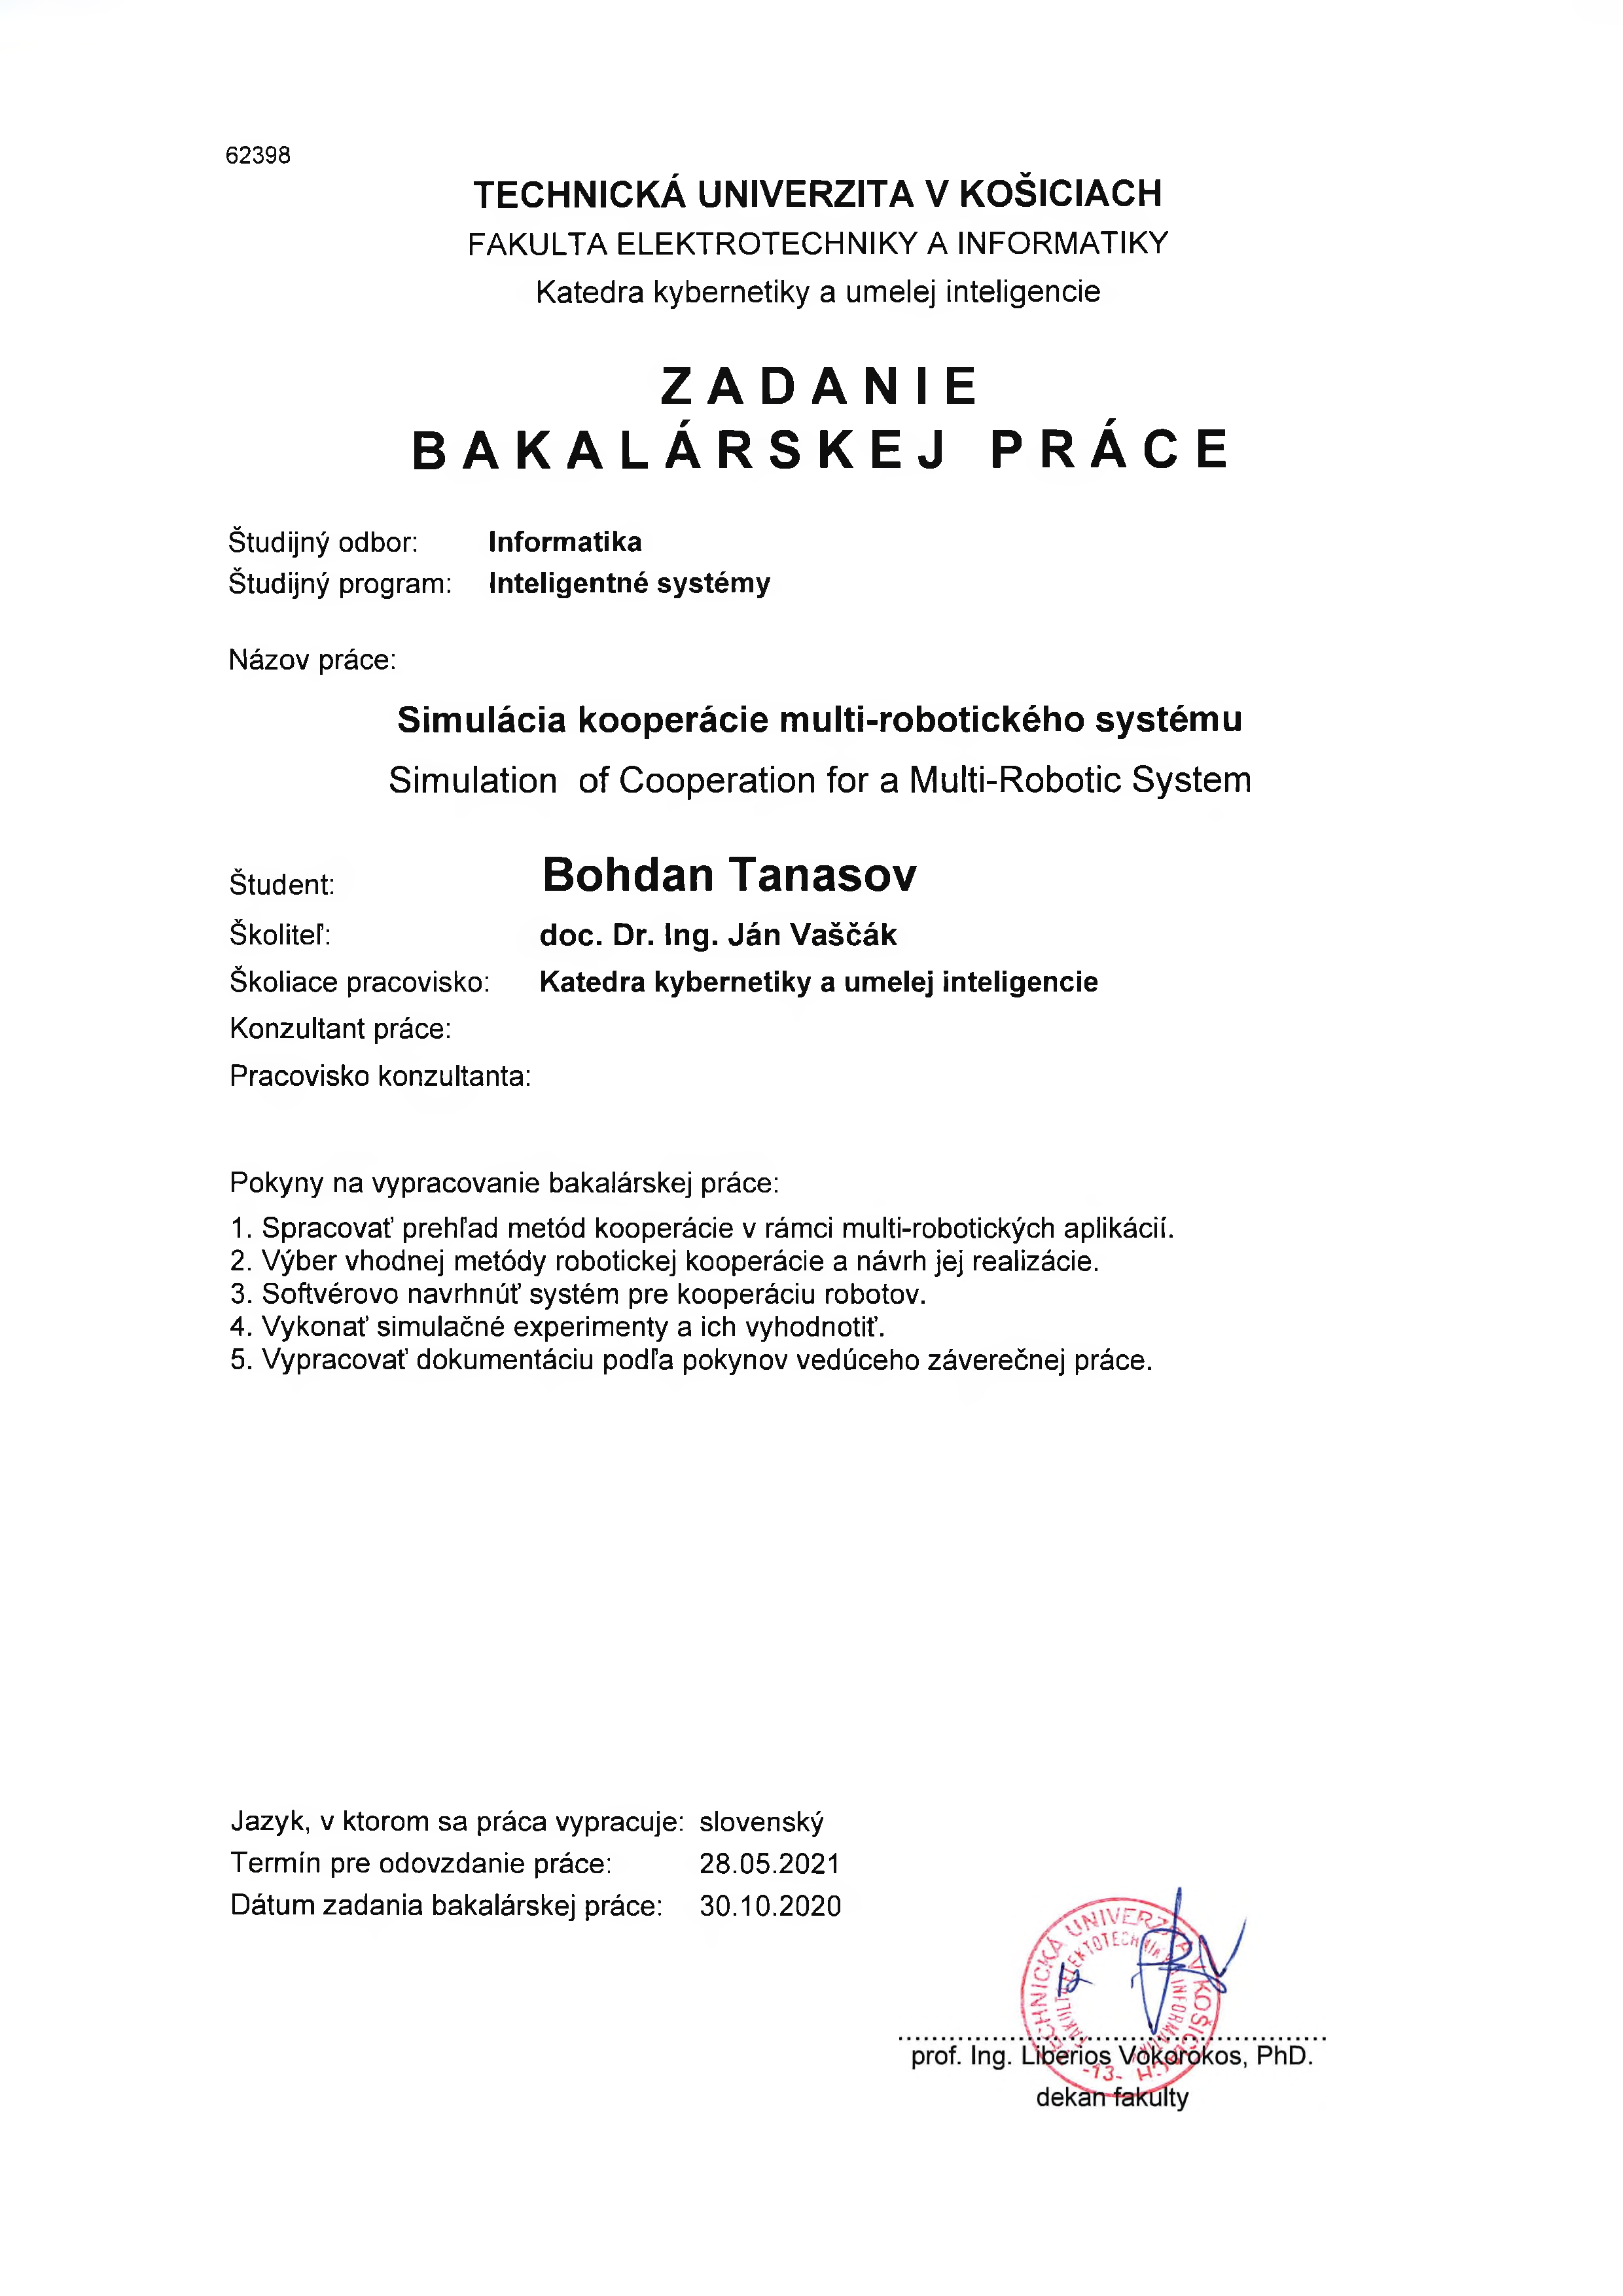
\includepdf[pages=-]{zadavaci-list.png}

\cestnevyhlasenie
% Niektorí autori metodických príručiek o~záverečných prácach sa
% nazdávajú, že takéto vyhlásenie je zbytočné, nakoľko povinnosť
% vypracovať záverečnú prácu samostatne, vyplýva študentovi zo zákona a
% na autora práce sa vzťahuje autorský zákon.

\podakovanie
Najskôr by som sa chcel poďakovať vedúcemu bakalárskej práce doc. Dr. Ing. Jánovi Vaščakovi. Príležitosť komunikovať s docentom Vaščakom bola vždy otvorená, kedykoľvek som narazil na problémové miesto alebo mal otázku o svojom výskume alebo písaní. Dôsledne pripúšťal, aby tato práca bola mojou vlastnou, ale vždy, keď si myslel, že to potrebujem, ma nasmeroval správnym smerom.

Na záver musím svojim rodičom poďakovať za to, že mi počas rokov štúdia a pri výskume a písaní tejto práce poskytovali neutíchajúcu podporu a neustále povzbudzovanie. Bez nich by tento úspech nebol možný. Ďakujem.
\kpodakovania

\predhovor
Účelom tejto práce je podrobne preskúmať niekoľko robotických systémov. Viaceré robotické systémy sú užitočné na vykonávanie úloh, ktoré by jeden robot ťažko splnil. V takom prípade je úlohou koordinovať niekoľko robotov v procese prenasledovania. Na prekonanie problémov, ktoré sa vyskytujú pri love, musí robot komunikovať. Roboty sú úplne autonómne a komunikujú bezdrôtovo. Cieľom projektu je demonštrovať užitočnosť koordinovaného správania v iných dôležitých aplikáciách. Získané praktické skúsenosti sa týkajú komunikácie, prideľovania úloh a učenia sa.
% Zvýšil sa záujem o výskum v systémoch zložených z viacerých autonómnych mobilných robotov vykazujúcich kooperatívne správanie. Konštruujú sa skupiny mobilných robotov s cieľom študovať také problémy, ako je skupinová architektúra, konflikt zdrojov, pôvod spolupráce, učenie sa a geometrické problémy. Doposiaľ bolo opísaných málo aplikácií kooperatívnej robotiky a teória podpory je stále v štádiu formovania. V tejto prace bol vytvorený multi-robotický projekt a diskutované problémy a variácie ich riešenia 
\kpredhovoru

\thispagestyle{empty}
\tableofcontents
\thispagestyle{empty}

\newpage

\thispagestyle{empty}

{	\makeatletter
	\renewcommand{\l@figure}{\@dottedtocline{1}{1.5em}{3.5em}}
	\makeatother
	\listoffigures}

%\addcontentsline{toc}{section}{\numberline{}Zoznam obrázkov}
%\listoffigures


\newpage

\thispagestyle{empty}
%\addcontentsline{toc}{section}{\numberline{}Zoznam tabuliek}
\listoftables

\thispagestyle{empty}
\newpage
 
\thispagestyle{empty}
%\addcontentsline{toc}{section}{\numberline{}Zoznam symbolov a
%skratiek}
\printglossary % vlozenie zoznamu skratiek a symbolov
\newpage

%\addcontentsline{toc}{section}{\numberline{}Slovník termínov}
\slovnikterminov

\begin{description}
	\item[Virtuálna štruktúra] je štruktúra tvorená a udržiavaná skupinou robotov, ktorí prenasledujú cieľ
	\item[\boldmath $R_p$] je zápis na diagramoch a obrázkoch robota Korisť
	\item[\boldmath $R_1, R_2, R_3$] je záznam o schémach a obrázkoch robotov zo skupiny prenasledovateľov
	\item[ROS] Robot Operating System.
	\item[Robot Korisť] je robot, ktorým ovláda človek pomocou klávesnice a jeho cieľom je utekať pred skupinou prenasledovateľov.	\item[Robot Prenasledovateľ] je hlavný robot zo skupiny prenasledovateľov.
	\item[r] konštantná minimálna vzdialenosť, na ktorú sa robot Prenasledovateľ nesmie priblížiť ku robotovi Korisť.
	\item[d(P,A)] je vzdialenosť od robota prenasledovateľa k robotovi koristi v konkrétnom čase.
	\item[R] je určitá konštantná bezpečná vzdialenosť od robota Korisť po robota Prenasledovateľ, ktorú sa skupina prenasledovateľov snaží udržať v sledovacom režime
	\item[\boldmath$l_x$] je vzdialenosť. 
\end{description}

\kslovnikterminov
%
% !TeX encoding = UTF-8
% !TeX spellcheck = sk_SK
% !TeX root=tukedip.tex

\section*{Úvod}
\addcontentsline{toc}{section}{\numberline{}Úvod}
\setcounter{page}{1}
Drony sa v posledných rokoch stávajú čoraz populárnejšími vďaka svojej schopnosti vykonávať širokú škálu úloh, ktoré by inak boli pre človeka náročné alebo nebezpečné. Schopnosť ovládať viacero dronov súčasne otvára ešte viac možností ich využitia. Na dosiahnutie tohto cieľa je potrebné vyvinúť riadiaci systém, ktorý umožní efektívne a intuitívne ovládanie viacerých dronov. Cieľom tejto práce je vyvinúť takýto systém pomocou webovej aplikácie React a socketov.

Navrhovaný riadiaci systém umožní používateľovi ovládať viacero dronov Tello súčasne pomocou webového rozhrania. Použitie značiek Aruco umožní dronom zistiť ich polohu a podľa nej sa navigovať, čo umožní ovládať drony v individuálnom aj skupinovom režime. Systém bude pozostávať z backendu Node.js, ktorý bude zabezpečovať komunikáciu medzi webovou aplikáciou a dronmi, ako aj z programu Python bežiaceho na doske Asus TinkerBoard pripojenej ku každému dronu. Každý dron bude mať špecifické ID, čo umožní ich rozlíšenie.

Vývoj takéhoto riadiaceho systému predstavuje niekoľko výziev vrátane potreby zvládnuť komunikáciu v reálnom čase medzi dronmi a webovou aplikáciou, potreby presne zistiť polohu dronov a potreby zabezpečiť, aby sa systém ľahko používal a poskytoval dobrý používateľský zážitok.

Navrhovaný systém má potenciál na využitie v rôznych aplikáciách, ako je napríklad sledovanie pomocou dronov, letecké fotografovanie alebo pátracie a záchranné operácie. Tým, že systém umožňuje efektívne a intuitívne ovládanie viacerých dronov, by mohol pomôcť zvýšiť bezpečnosť a efektívnosť týchto operácií.

Zvyšok tejto práce je usporiadaný takto. V časti 2 sa uvádza prehľad príslušných technológií a metód, ktoré boli použité pri vývoji systému. V časti 3 je opísaný proces vývoja riadiaceho systému vrátane krokov vykonaných pri návrhu, implementácii a testovaní systému. V časti 4 sú uvedené výsledky práce vrátane podrobného opisu vyvinutého systému, jeho vlastností, používateľského rozhrania a funkčnosti, ako aj ukážky možností systému prostredníctvom príkladov použitia. V časti 5 sa hodnotí výkonnosť a použiteľnosť systému pomocou príslušných metrík a spätnej väzby od používateľov. Nakoniec sa v oddiele 6 uvádza zhrnutie výskumnej otázky, cieľov a prínosov, ako aj diskusia o obmedzeniach systému a možných cestách pre budúcu prácu a zlepšenie.
%
% !TeX encoding = UTF-8
% !TeX spellcheck = sk_SK
% !TeX root=tukedip.tex
\section{Formulácia úlohy}
\textbf{Spracovať prehľad metód kooperácie v rámci multi-robotických aplikácií.} Táto časť bakalárskej práce obsahuje popis úloh, ktoré sa riešia pri vzájomnej interakcii viacerých robotov. 
Táto kapitola obsahuje prehľad robotov, kontrolné metódy, komunikačné metódy a problémy, ktoré sa vyskytujú pri vývoji algoritmov pre multi-robotický systém.\newline\newline
% \bigskip
\textbf{Výber vhodnej metódy robotickej kooperácie a návrh jej realizácie.} Táto časť popisuje proces výberu najvhodnejšej metódy na implementáciu 
multi-robotického projektu na základe výhod a nevýhod rôznych metód uvedených v predchádzajúcej časti.\newline\newline
% \bigskip
\textbf{Softvérovo navrhnúť systém pre kooperáciu robotov. } Táto časť bude obsahovať prehľad softvéru potrebného na vypracovanie bakalárskeho projektu a tiež popis metód a prístupov použitých pri práci na projekte.\newline\newline
% \bigskip
\textbf{Vykonať simulačné experimenty a ich vyhodnotiť. } Táto kapitola predstavuje výsledky a vyhodnotenie simulačných experimentov vykonaných pre rôzne situácie. Každá simulácia má svoj vlastný popis a ku každej je pridaný záver\newline\newline
% \bigskip
\textbf{Vypracovať dokumentáciu podľa pokynov vedúceho záverečnej práce.} Posledný bod bude súvisieť s prípravou dokumentácie a popisom celého procesu vývoja tohto projektu. 

%
% !TeX root=tukedip.tex
% !TeX encoding = UTF-8
% !TeX spellcheck = sk_SK
\section{Metódy riadenia v multi-robotických systémoch}
V organizácii a správe systémov s niekoľkými mobilnými robotmi v súčasnosti existuje veľa rôznych prístupov. Nedá sa povedať, že existujú správne alebo nesprávne prístupy, každý zo systémov má svoje výhody aj nevýhody. Rozhodnutie o použití systému sa prijíma na základe konkrétnej úlohy projektu.
V tejto časti sa pozrieme na rôzne metódy riadenia a organizácie multi-robotických systémov, ako aj na ich výhody a nevýhody.

\subsection{Multi-robotické systémy}

Systémy viacerých robotov sú dobré z mnohých ďalších dôvodov. Podľa Aparicio a Lima \citep{aparicio} systémy s viacerými robotmi  ponúkajú robustnosť a prispôsobivosť, aké sa v systémoch s jedným robotom nenachádzajú. Ak je jeden agent v systéme poškodený alebo nefunguje správne, je možné úlohu dokončiť so zvyšnými agentmi. Túto myšlienku možno uplatniť aj pri údržbe. Agenti môžu byť obsluhovaní po jednom, čo vedie k skutočnosti, že systém nie je nečinný, ak sú ostatní roboti schopní pokračovať v plnení úlohy bez prítomnosti ich partnera. Viaceré roboty navyše dokážu pokryť veľkú oblasť a môžu sa špecializovať na menšie úlohy, ktoré postupujú k splneniu väčšej úlohy \citep{aparicio}. Preto je pravdepodobnejšie, že systémy s viacerými robotmi budú spoľahlivo vykonávať veľké a zložité úlohy. Napriek mnohým výhodám systémov viacerých robotov je potrebné vyriešiť niekoľko nevýhod. Najskôr je komunikácia medzi agentmi v systéme výpočtovo zložitá. Podľa Coesa, Nurbakhsh a Sikar %\citep{koes} 
, keď sa systémy s viacerými robotmi rozhodnú, musia brať do úvahy čas potrebný na cestu na konkrétne miesto, čas čakania na príchod ďalších robotov a čas na dokončenie úlohy. V dôsledku toho sú riadiace algoritmy veľmi zložité, pretože systém sa implementuje ťažšie, ak na konkrétnom probléme pracuje viac agentov. Rádiová komunikácia dodáva systému ďalšiu vrstvu zložitosti, pretože si vyžaduje použitie prenosových obvodov a komunikačných protokolov. Preto, aj keď môže byť systém s viacerými robotmi efektívnejší, tento však vyžaduje väčšiu zložitosť než systém s jedným robotom. 

\subsection{Praktické využitie multi-robotických systémov}

Počas výskumu boli objavené aplikácie, ktoré priamo súvisia s mojím projektom. V jednom konkrétnom príklade boli na
premiestnenie nábytku na konkrétne miesta použité dva veľké roboty. V praktickejšom príklade je možné použiť roboty na
presun ťažkých materiálov na stavenisku. Je pravdepodobné, že roboty s takouto úlohou veľmi pomôžu a môžu zvýšiť
efektivitu, ale roboty sú zvyčajne príliš drahé na to, aby boli finančné prospešné.
\vspace{3mm}

\justifying
\noindent 
Jednou z možností v súčasnosti je použitie koordinovaných robotov na skúmanie oblastí, ktoré by mohli byť pre
človeka nebezpečné. Tieto roboty môžu autonómne zvyšovať bezpečnosť alebo vytvárať nebezpečné oblasti. Napríklad oblasť
plná mín môže byť vhodná pre robotov vybavených senzormi určenými na detekciu mín. Potom, čo v mínovom poli, bude robot schopný rozpoznať mínu bez účasti ľudí. nájdení bane môže robot oznámiť polohu míny ďalším robotom.
Ostatní roboti pomocou koordinačných algoritmov a pozičných senzorov budú môcť k míne pristúpiť a pomôcť ju rozobrať
alebo označiť. Roboti sa môžu navzájom rozprávať alebo môžu používať hlavného robota, ktorý dáva každému z nich smer
\citep{mclurkin}. Projekt, ktorý je rovnako jednoduchý ako koordinované tlačenie škatúľ robotom, slúži ako východiskový bod pre
zložitejší a užitočnejší systém, ako sú napríklad robotické vyhľadávače mín.

\subsection{Ovládanie multi-robotických systémov}
Ovládanie systému s viacerými robotmi je vo všeobecnosti náročným problémom. K tejto otázke existujú dva prístupy:
centralizovane riadenie a decentralizovane riadenie \citep{kexu}.

\subsubsection{Centralizovaný systém}
V centralizovanom systéme s niekoľkými robotmi sa ukladajú globálne informácie o stave celého systému. Systém
zhromažďuje informácie o všetkých robotoch a sleduje ich polohu v prostredí. Na základe informácií získaných od robotov
dokáže zostaviť mapu. Tento systém je buď na stacionárnom hostiteľovi, alebo v jednom robote, ktorý zjavne funguje ako
hlavný. Potom majster zorganizuje tím robotov, aby dosiahli spoločný cieľ a naplánuje úlohy pre jednotlivých členov tímu
a dohliada na celý proces.
Táto architektúra sa dá ľahko navrhnúť, ale nie je odolná voči výpadkom komunikácie a nepredvídateľným situáciám.
Centralizované riadenie je zvyčajne vhodné pre obmedzený počet robotov, ktorí pracujú v známom a nemennom prostredí.

\subsubsection{Decentralizovaný systém}
Naproti tomu decentralizované systémy nezahŕňajú žiadneho riaditeľa, ktorý má úplné informácie o stave systému a riadi
celý proces. Naopak, každý robot je autonómna jednotka, ktorá koná v súlade so stavom svojho prostredia. Robot si je
samozrejme vedomý prítomnosti ďalších robotov a môže s nimi komunikovať na miestnej úrovni. Komplexné skupinové
správanie vyplýva z interakcií medzi robotmi a prostredím. Táto architektúra je veľmi robustná, môže dobre fungovať v
nepriateľskom prostredí a je škálovateľná, potenciálne obrovské množstvo homogénnych robotov môžu spolupracovať na
dosiahnutí spoločného cieľa.

\subsection{Problématika riadenia}
Problém s riadením v navigácii mobilných robotov sa rieši dvoma spôsobmi: deliberatívnym a reaktívnym riadením (Obrázok 2 –
1).

\begin{figure}[ht!]
    \centering
    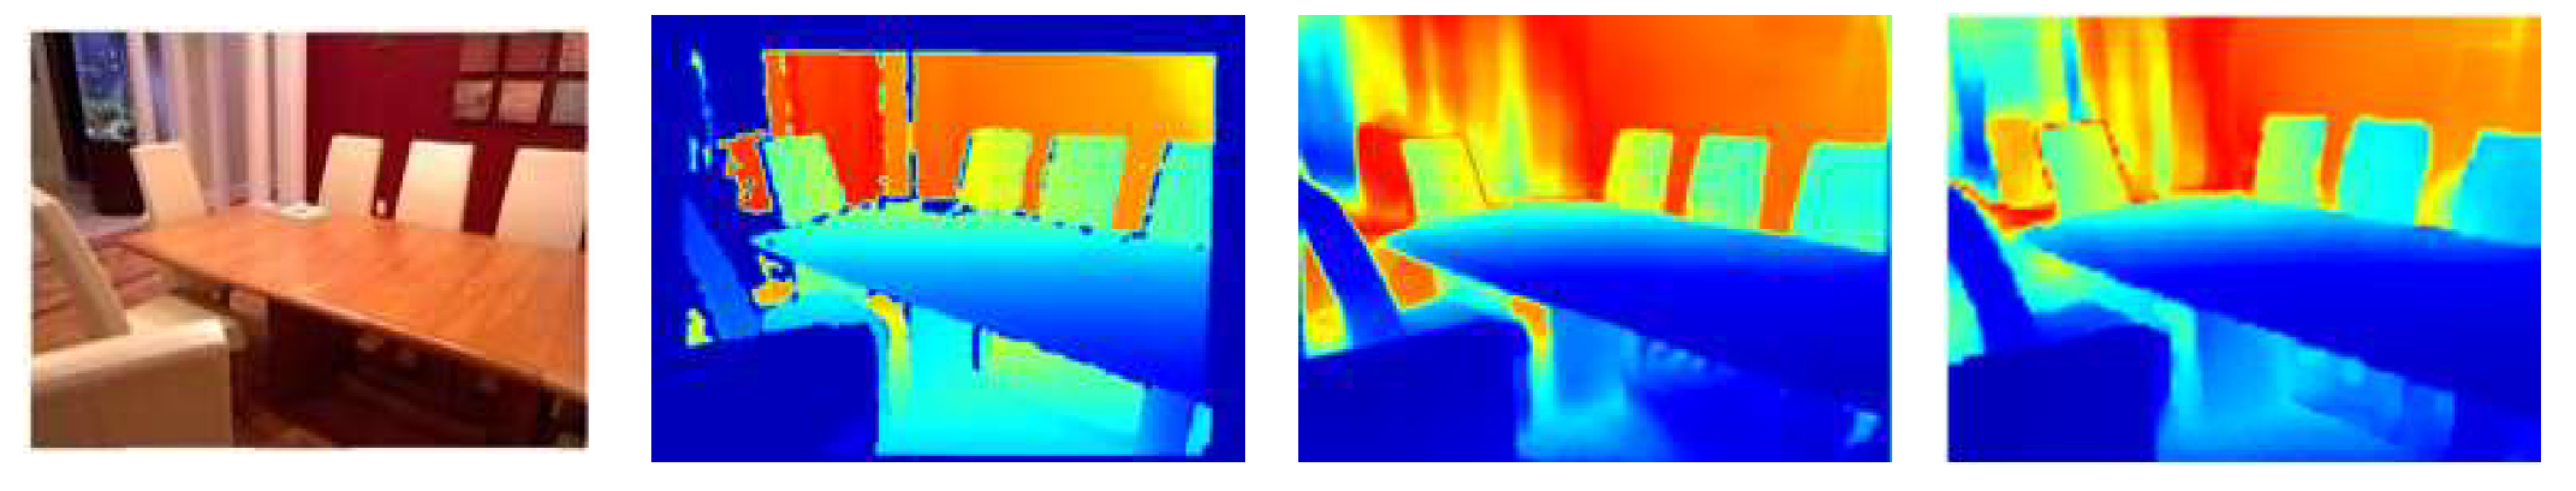
\includegraphics[width=.85\textwidth,angle=0]{figure 2-1.pdf}
    \caption{Stratégie riadenia navigácie v formácií.}
    \label{o:3}
\end{figure}

\subsubsection{Deliberatívne riadenie}
Prístup založený na plánovaní pohybu a trajektórie pohybu vyžaduje predbežné znalosti prostredia na plánovanie pohybov
robotov \citep{vascak}. Tento prístup využíva formalizmy ako Voronoiove diagramy alebo umelé potenciálne funkcie \citep{rimon},
pričom zohľadňuje všeobecné poznatky o životnom prostredí. Plánovanie pohybu je všeobecne optimálne z hľadiska
efektívnosti / reaktivity. V skutočnosti sa pre mierku veľmi veľkého počtu robotov nemodifikujú dobre kvôli výpočtovej
zložitosti. Vďaka predchádzajúcim znalostiam prostredia však roboti svoju misiu zvyčajne úspešne dokončia dobrým
výkonom.

\subsubsection{Reaktívne riadenie}
Pri reaktívnej metóde, roboty konajú iba podľa informácií svojich miestnych senzorov bez akýchkoľvek
ďalších všeobecných znalostí. Techniky založené na správaní sú vynikajúcou ilustráciou reaktívnej kontroly.
Globálna úloha robota je v skutočnosti rozdelená na súbor čiastkových úloh (vzorce správania).
Podľa informácií o senzore je stratégia riadenia použitá na robota založená na jednom zvolenom vzorci správania 
alebo je zlúčením niekoľkých vážených modelov. Keď aplikácia vyžaduje, aby roboty fungovali v reálnom čase (napríklad v nebezpečných
prostrediach), je zrejmé, že reaktívne metódy sa stávajú oveľa zaujímavejšími ako plánovanie pohybu \citep{vascak}.

\paragraph{Hierarchická stratégia.}
Pri prvom prístupe sa jeden alebo viac robotov považuje za vedúcich a iné roboti sú ďalší. Vedúci typicky sleduje danú
trajektóriu, zatiaľ čo nasledovníci sledujú jej transformované súradnice. Tento prístup sa dá ľahko sledovať.
Je však zaznamenané, že problém s hlavným robotom spôsobí zastavenie celého systému. V prístupe distribuovaného správania, 
neexistuje medzi robotmi hierarchia. Každý má svoje vlastné vnímanie a kontrolu a porucha robota nevedie k zlyhaniu
skupiny \citep{vascak}.

\paragraph{Stratégia správania.}
Stratégia založená na správaní znamená, že každý robot má súbor správania (základné úlohy), ktoré musia byť vykonané.
Výsledné skupinové správanie vyplýva zo základnej lokálnej interakcie bez explicitného vzoru celkového kooperatívneho
správania. Tento prístup však bol kritizovaný za to, ako volí riadenie pre každého robota. Podľa informácií o vnímaní
riadiaci systém v skutočnosti prepína medzi správaním (napríklad konkurenčný prístup) alebo kombinuje niekoľko
ovládačov (napríklad motorický obvod). To prirodzene sťažuje štúdium udržateľnosti stratégie globálneho riadenia \citep{ogren}.

\paragraph{Stratégia virtuálnej štruktúry.}
Virtuálna štruktúra (tretí prístup) považuje vzdelávanie za jediné virtuálne telo. Tvar posledného menovaného je
požadovaný tvar formácie a jeho pohyb sa prevedie na požadovaný pohyb každého vozidla. Virtuálna štruktúra
bola implementovaná v niekoľkých dielach s využitím potenciálnych metód poľa: teda všetky prvky formácie
sledujú pridelené uzly, ktoré prechádzajú do požadovanej konfigurácie. Na rozdiel od plánovania
pohybu využívajú potenciálne funkcie použité pri prístupe k virtuálnej štruktúre iba okamžité a lokálne vnímanie
robotov. Nedostatočné využitie potenciálnych prvkov pre tento druhý prístup zodpovedá zvyšujúcej sa zložitosti riadenia
tvaru flotily v dynamickom prostredí. To v skutočnosti znamená, že robot je vystavený často sa meniacemu počtu /
amplitúde síl, čo vedie k ďalším lokálnym minimám, fluktuáciám atď. Preto je v tomto prípade veľmi ťažké preukázať
spoľahlivosť a stabilitu navigácie \citep{ogren}, \citep{vascak}.



\subsection{Multi-robotické systémy podľa typovosti}
Skupinu robotov definujeme ako homogénnu, ak sú možnosti jednotlivých robotov rovnaké a inak skupina je heterogénna. Heterogenita
vo všeobecnosti prináša zložitosť, pretože alokácia úloh sa stáva zložitejšou a agenti majú väčšiu potrebu modelovať
ďalších robotov v skupine. Existuje koncept pokrytia úlohy, ktorý meria schopnosť daného člena tímu dosiahnuť danú
úlohu. Tento parameter predstavuje index dopytu po spolupráci: keď je pokrytie úloh vysoké, úlohy je možné splniť bez
väčšej spolupráce, ale inak je spolupráca nevyhnutná. Pokrytie úlohy je maximálne v homogénnych skupinách a klesá, keď
sú skupiny čoraz viac heterogénne (t. j. v krajnom prípade môže danú úlohu vykonať iba jeden agent v skupine).
V literatúre v súčasnosti prevládajú diela, ktoré predpokladajú homogénne skupiny robotov. Niektoré pozoruhodné
architektúry však dokážu zvládnuť heterogenitu, napr. ACTRESS a ALLIANCE. V heterogénnych
skupinách môže byť alokácia úloh určená individuálnymi schopnosťami, ale v homogénnych systémoch môže byť potrebné, aby
sa agenti diferencovali do rôznych rolí, ktoré sú vždy známe v čase návrhu alebo dynamicky vznikajú za behu \citep{vascak}.

\subsection{Komunikačné štruktúry}
Komunikačná štruktúra skupiny určuje možné spôsoby interakcie. Charakterizujeme tri základné typy interakcií, ktoré môžu
byť podporované.

\subsubsection{Interakcia prostredím}
Najjednoduchší typ interakcie sa vyskytuje, keď je samotné prostredie komunikačné médium (v skutočnosti,
zdieľanej pamäti) a medzi agentmi nie je explicitná komunikácia alebo interakcia. Niektorí výskumníci tiež nazývali túto
modalitu s "spoluprácou bez komunikácie" \citep{arkin}.

\subsubsection{Interakcia prostredníctvom snímania}
Interakcia prostredníctvom snímania patrí do miestnych interakcií, ktoré sa vyskytujú medzi agentami v dôsledku toho, že agenti sa navzájom cítia, ale bez
explicitnej komunikácie. Tento typ interakcie si vyžaduje schopnosť agentov rozlišovať medzi inými činiteľmi v skupine a
ďalších objektoch v prostredí, ktoré sa v niektorých literárnych zdrojoch nazýva "súvisiace uznanie" \citep{mataric}.
Interakcia prostredníctvom sondovania je potrebná na simuláciu iných agentov. Vzhľadom na obmedzenia hardvéru je
interakcia cez snímanie často emulovaná pomocou rádiovej alebo infračervenej komunikácie.

\subsubsection{Interakcia prostredníctvom komunikácie}
Tretia forma interakcie spočíva v explicitnej komunikácii s inými agentmi buď prostredníctvom zmenených, alebo
vysielaných zámerných správ (príjemca správy môže byť známy alebo neznámy). Pretože architektúry,
ktoré umožňujú túto formu komunikácie, sú podobné komunikačným sieťam, vzniká veľa štandardných problémov z oblasti
sietí, vrátane návrhu sieťových topológií a komunikačných protokolov. Napríklad na komunikáciu medzi robotmi
môže sa použiť prístupový protokol k médiám (podobný protokolu Ethernet). Aj som stretol komunikáciu pomocou protokolu
„hello-call“, pomocou ktorého ustanovujú „reťazce“ s cieľom rozšíriť svoje
efektívne komunikačné rozsahy a bezdrôtovým protokolom CSMA/CD (Carrier Sense Multiple Access with Collision Detection)
pre distribuované robotické systémy \citep{wang}.

\subsection{Vybrané typy architektúr}
Všetky systémy implementujú určitú skupinovú architektúru. Teraz popíšeme niekoľko obzvlášť dobre definovaných
reprezentatívnych architektúr spolu s prácami vykonanými v každom z ich rámcov. Je zaujímavé poznamenať, že tieto
architektúry zahŕňajú celé spektrum od tradičnej AI po vysoko decentralizované prístupy.

\subsubsection{CEBOT}
CEBOT (CEllular roBOTics System) je decentralizovaná, hierarchická architektúra inšpirovaná bunkovou organizáciou
biologických entít. Systém sa konfiguruje dynamicky  v tých základných autonómnych „bunkách“ (robotoch), ktoré je
možné fyzicky spojiť s inými bunkami, a dynamicky konfigurujú svoju štruktúru na „optimálnu“ konfiguráciu v reakcii na
meniace sa prostredia. V hierarchii CEBOT existujú „hlavné bunky“, ktoré koordinujú čiastkové úlohy a komunikujú s
ostatnými hlavnými bunkami \citep{michael} \citep{beatriz}.

\subsubsection{ACTRESS}
V systéme ACTRESS (robot a syntetický systém na báze ACTor) tvoria „roboti“ vrátane 3 robotov a 3 pracovných staníc
(jeden ako rozhranie k ľudskému operátorovi, jeden ako obrazový procesor a druhý ako globálny manažér prostredia)
heterogénnu skupinu, ktorá sa snaží vykonávať úlohy, ako je tlačenie objektov, ktoré nemôže vykonať žiadny z
robotov sám. Komunikačné protokoly na rôznych úrovniach abstrakcie poskytujú prostriedky, na ktorých
sú postavené mechanizmy „skupinového obsadenia“ a rokovacie mechanizmy založené na viacstupňových protokoloch vyjednávania. Študujú sa rôzne problémy, ako napríklad efektívna komunikácia medzi robotmi a manažérmi
prostredia, predchádzanie kolíziám \citep{beatriz}.

\subsubsection{SWARM}
SWARM je distribuovaný systém s veľkým počtom autonómnych robotov. (Upozorňujeme, že práca na systémoch SWARM sa
začala ako práca na bunkových robotických systémoch, kde mnoho jednoduchých agentov obsadzovalo jedno- alebo
dvojrozmerné prostredie a boli schopní vykonávať úlohy, ako je generácia vzorov a samoorganizácia). Inteligencia SWARM
je „vlastnosťou systémov neinteligentných robotov vykazujúcich kolektívne inteligentné správanie“. Samoorganizácia
v SWARM-e je schopnosť distribuovať sa „optimálne“ pre danú úlohu, napríklad prostredníctvom formovania geometrických
vzorov alebo štruktúrnej organizácie. SWARM vykazuje distribuovanú architektúru, zvyčajne bez rozdielov medzi členmi.
Interakcia prebieha tak, že každá bunka reaguje na stav \citep{beatriz}.

\subsubsection{GOFER}
Architektúra GOFER bola použitá na štúdium distribuovaného riešenia problémov viacerými mobilnými robotmi vo
vnútornom prostredí s využitím tradičných techník AI. V systéme GOFER centrálny systém plánovania a plánovania úloh
(CTPS) komunikuje so všetkými robotmi a má globálny prehľad o úlohách, ktoré sa majú vykonať, aj o dostupnosti robotov
na vykonávanie úloh. CTPS generuje štruktúru plánu (šablóna pre inštanciu plánu) a informuje všetkých dostupných robotov
o očakávaných cieľoch a štruktúrach plánu. Roboty používajú na určenie svojich rolí algoritmus prideľovania úloh \citep{caloud}.

\subsubsection{ALLIANCE}
Architektúru ALLIANCE vyvinul Parker \citep{parek} s cieľom študovať spoluprácu v heterogénnom, malom až strednom tíme
prevažne nezávislých a voľne prepojených robotov. Roboty sa považujú za schopné s určitou pravdepodobnosťou vycítiť
účinky ich vlastných činov a činov iných agentov prostredníctvom vnímania a explicitnej rozhlasovej komunikácie.
Jednotliví roboti sú založené na ovládači založenom na správaní s rozšírením pre aktiváciu „skupín správania“, ktoré
plnia určité úlohy. Tieto súbory sú aktivované motivačným správaním, ktorého aktivity sú určené robotovou
informovanosťou ich spoluhráčov \citep{beatriz} \citep{vascak}.


%   
% !TeX encoding = UTF-8
% !TeX spellcheck = sk_SK
% !TeX root=tukedip.tex

\section{Implementácia projektu}
V tejto časti podrobne opíšeme realizáciu nášho projektu. Opíšeme architektúru systému a účel jednotlivých modulov. Poskytneme aj prehľad štruktúry kódu a funkčnosti jednotlivých súborov. Okrem toho vysvetlíme, ako sme do nášho projektu integrovali rôzne technológie a knižnice, aby sme dosiahli naše ciele. Nakoniec rozoberieme všetky problémy, s ktorými sme sa stretli počas procesu implementácie, a ako sme ich riešili.
\subsection{Prehľad štruktúry programov} 

    \begin{center}
        \begin{tikzpicture}[node distance=3cm]
            \node (main) [draw, rectangle] {main.py};
            \node (tello) [draw, rectangle, below of=main] {tello.py};
            \node (cam) [draw, rectangle, right of=main, xshift=2cm] {cam\_class.py};
            \node (targeter) [draw, rectangle, right of=cam, xshift=2cm] {targeter.py};
            \node (video) [draw, rectangle, below of=tello] {video\_writer.py};
            \node (marker) [draw, rectangle, below of=cam] {marker\_class.py};
            \node (pid) [draw, rectangle, below of=targeter] {pid.py};
            \node (transform) [draw, rectangle, below of=marker] {transformations.py};

            \draw[-latex] (main) -- (tello);
            \draw[-latex] (tello) -- (main);
            \draw[-latex] (main) -- (cam);
            \draw[-latex] (cam) -- (main);
            \draw[-latex] (cam) -- (targeter);
            \draw[-latex] (targeter) -- (cam);
            \draw[-latex] (targeter) -- (pid);
            \draw[-latex] (pid) -- (targeter);
            \draw[-latex] (tello) -- (video);
            \draw[-latex] (cam) -- (marker);
            \draw[-latex] (marker) -- (transform);
            \draw[-latex] (transform) -- (marker);
        \end{tikzpicture}
    \end{center}

    \textbf{Popis:}

    \textbf{main.py} - Obsahuje grafické rozhranie pyGame a zobrazenie obrazu kamery. Používa rôzne klávesy na klávesnici na prepínanie funkcií alebo ovládanie dronu.

    \textbf{tello.py} - Obsahuje funkcie na komunikáciu s dronom a čítanie údajov.

    \textbf{video\_writer.py} - Beží na samostatnom vlákne, zachytáva video počas automatického ovládania a potom ho vypúšťa.

    \textbf{cam\_class.py} - Vykonáva úlohy spracovania obrazu (kalibrácia, rozpoznávanie značiek) a údaje o rýchlosti dronu sa odtiaľto zaraďujú do frontu. Odovzdáva načítané pozície značiek funkciám, ktoré ich spracúvajú.

    \textbf{targeter.py} - Prečíta funkcie zodpovedajúce poradovým číslam značiek zo zadaného súboru CSV a vráti vektor kontrolnej základne.

    \textbf{pid.py} - Obsahuje triedu implementujúcu numerický PID regulátor, vypočítava hodnoty regulačného stupňa.

    \textbf{marker\_class.py} - Trieda, ktorá uchováva všetky údaje pre značky. Počas zberu údajov počíta a nakoniec zapisuje zozbierané pozície do súboru NPZ.
 
    \textbf{transformations.py} - Implementuje transformácie súradnicového systému a obsahuje funkcie na konverziu vektorov rotácie.

 
\subsection{Ovládanie drona}
Dron Tello sa ovláda pomocou kombinácie softvérových programov, ktoré s ním komunikujú prostredníctvom pripojenia Wi-Fi (obrázok 4-1). Na nízkoúrovňovú komunikáciu medzi dronom a riadiacim počítačom sa používa knižnica Tello Python, tello.py.

\begin{figure}[ht!]
    \centering
    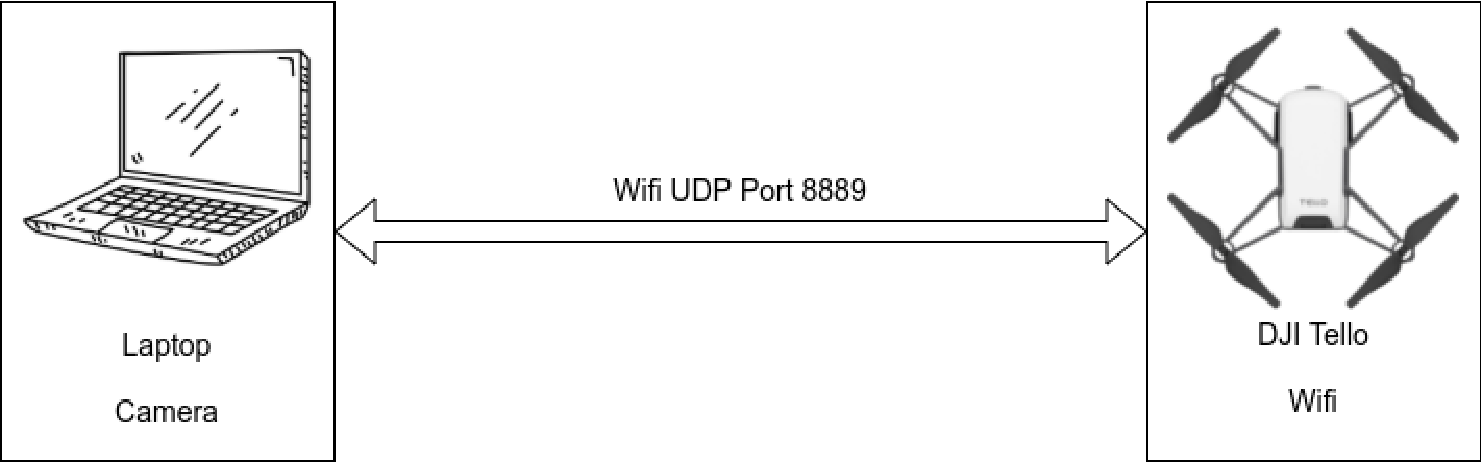
\includegraphics[width=.70\textwidth,angle=0]{figure 4-3.pdf}
    \caption{Schéma procesu pripojenia dronu.}
    \captionsetup{font=footnotesize, justification=centering, skip=5pt}
    \caption*{(Zdroj: vlastné spracovanie)}
    \label{o:4-3} 
\end{figure}  

Knižnica tello.py poskytuje množstvo funkcií, ktoré možno použiť na odosielanie príkazov do dronu a prijímanie údajov z neho. Medzi tieto funkcie patria 
$takeoff()$, $land()$, $move\_left()$, $move\_right()$, $move\_forward()$, $move\_backward()$, \break $rotate\_clockwise()$, $rotate\_counter\_clockwise()$ 
a mnohé ďalšie. Knižnica obsahuje aj funkcie na získavanie údajov z dronu, ako je jeho aktuálna výška, úroveň nabitia batérie a čas letu.

Na ovládanie dronu Tello z webovej aplikácie program využíva spojenie "web-sockets" na komunikáciu so skriptom Python na strane servera. Tento skript funguje ako most medzi webovou aplikáciou a dronom Tello a prenáša medzi nimi príkazy a údaje.

Skript na strane servera používa knižnicu tello.py na odosielanie príkazov do dronu a prijímanie údajov z neho. Keď používateľ zadá príkaz vo webovej aplikácii, príkaz sa odošle na server prostredníctvom spojenia "web-sockets". Server potom použije príslušnú funkciu v knižnici tello.py na odoslanie príkazu dronu. Po vykonaní príkazu môže server získať všetky relevantné údaje z dronu a poslať ich späť do webovej aplikácie na zobrazenie.

Celkovo kombinácia tello.py a skriptu na strane servera poskytuje výkonnú platformu na ovládanie dronu Tello z webovej aplikácie. Vďaka možnosti odosielať širokú škálu príkazov a získavať podrobné údaje z dronu.

\subsection{Spracovanie obrázkov}
S riadením dronov úzko súvisí, ale viac sa zaoberá spracovaním obrazu, program cam\_class.py, ktorého hlavná funkcia je zodpovedná za rozpoznávanie značiek ArUco. ArUco značky sa zisťujú pomocou vstavanej funkcie OpenCV cv2.aruco.detectMarkers(). Tá nájde kódy v načítanom zväzku značiek po adaptívnej segmentácii aplikovanej na obraz v odtieňoch sivej a vráti ich rohové body v pixeloch a ich poradové číslo. Na výpočet skutočnej trojrozmernej polohy značiek na základe matíc kamery sa používa už spomínaná transformácia PnP. Výsledné polohy s ich poradovým číslom značky sa môžu odoslať na ďalšie spracovanie (časť 4.4) alebo použiť na automatickú navigáciu dronu.

Program je určený na navigáciu dronu Tello pomocou značiek umiestnených na zemi. To sa dosiahne použitím knižnice OpenCV na detekciu značiek vo videozázname z kamery dronu.
\begin{mypython}[caption={Inicializácia parametrov detekcie značiek OpenCV},label=CL-3]

    import cv2
    import numpy as np
    from djitellopy import Tello
    
    # Initialize Tello drone
    tello = Tello()
    tello.connect()
    tello.streamon()
    
    # Initialize OpenCV marker detection parameters
    aruco_dict = cv2.aruco.Dictionary_get(cv2.aruco.DICT_6X6_250)
    aruco_params = cv2.aruco.DetectorParameters_create()
    
    # Set up video stream
    stream = tello.get_video_stream()
\end{mypython}

Program najprv inicializuje kameru a nastaví tok videa. Potom pomocou slučky nepretržite zachytáva snímky z videoprenosu a spracováva ich. Pre každú snímku program používa vstavané funkcie OpenCV na detekciu značiek a odhad ich polohy v 3D priestore.
\begin{mypython}[caption={Detekcia značky a vypočítanie polohy},label=CL-4]
    while True:
    # Capture frame from video stream
    frame = stream.read()

    # Detect markers in frame
    corners, ids, rejected = cv2.aruco.detectMarkers(frame, aruco_dict, parameters=aruco_params)

    # Estimate marker position in 3D space
    rvecs, tvecs, _ = cv2.aruco.estimatePoseSingleMarkers(corners, 0.05, camera_matrix, dist_coeffs)

    # Process marker positions
    if ids is not None:
        # TODO: Implement control algorithm
        pass

    # Display frame
    cv2.imshow('Frame', frame)
    if cv2.waitKey(1) & 0xFF == ord('q'):
        break

\end{mypython}

Po odhadnutí polohy značiek program pomocou proporcionálneho riadiaceho algoritmu upravuje odklon, sklon a výšku dronu na základe polohy značiek vzhľadom na stred snímky. Algoritmus vypočíta chybu medzi stredom rámu a polohou značiek a upraví orientáciu a výšku dronu tak, aby sa táto chyba minimalizovala.

Program obsahuje aj niekoľko bezpečnostných funkcií, ktoré zabraňujú kolízii dronu s prekážkami alebo vyleteniu mimo dosahu. Medzi tieto funkcie patrí nastavenie maximálnej výšky a doletu dronu, ako aj detekcia prekážok v dráhe dronu a automatické nastavenie jeho trajektórie tak, aby sa im vyhol.

Na ďalšie zlepšenie presnosti a spoľahlivosti detekcie a sledovania značiek program obsahuje množstvo konfigurovateľných parametrov, ako je minimálna a maximálna veľkosť značky, prah detekcie a proporcionálne zisky riadenia. Tieto parametre sa dajú upraviť tak, aby sa optimalizoval výkon programu pre rôzne prostredia a svetelné podmienky.

Celkovo program poskytuje spoľahlivý a efektívny spôsob navigácie dronu Tello pomocou značkovačov. Použitím knižnice OpenCV na detekciu a sledovanie značiek v reálnom čase a implementáciou proporcionálneho riadiaceho algoritmu na úpravu orientácie a výšky dronu je program schopný navigovať dron s vysokou mierou presnosti a precíznosti.

\subsection{Spracovanie údajov}
Spracovanie priestorových bodov a rotácií získaných z programov na spracovanie obrazu z kamery, t. j. zber údajov, vykonáva program marker\_class.py. Potrebné transformácie, ktoré sú opísané vyššie, vykonávajú funkcie transformations.py.
\subsubsection{Ukladanie údajov o značkách}
Na spracovanie sa môžu odovzdať len údaje značiek, ktoré nemajú žiadny zo svojich vrcholov v pixelovom rámci obrazu. Definícia hrany je 2-2-2-2 \% priesečník na všetkých štyroch stranách obrazu kamery. Značkovače umiestnené na okrajoch poskytujú po odstránení skreslenia jednak nepresnejšie údaje, jednak môžu spôsobiť neistotu označenia vonkajších okrajov 2D kódu značkovača počas detekcie značkovača, ako je to vidieť na obrázku 20.
%TODO: obrazok

V triede markers sú vlastnosti značiek, ktoré ste doteraz videli, uložené v rôznych zoznamoch, ako napríklad:
\begin{itemize}
    \item \textbf{ids}: počet už použitých značiek
    \item \textbf{tvec\_origin}: "markerorigos" v globálnom súradnicovom systéme
    \item \textbf{rvec\_origin}: otočenie súradnicového systému značiek vzhľadom na globálny
    \item \textbf{dRot}: matica rotácie od danéj značky ku globálnemu.
    \item \textbf{allow\_use}: pomocná premenná, ktorá umožňuje použitie danéj značky pri priemerovaní, akonáhle sa zozbiera dostatočný počet vzoriek, môže sa započítať
    \item \textbf{tvec\_min, tvec\_max}: pomocné premenné na filtrovanie výpočtu priemeru
\end{itemize}

Funkcia appendMarker() volaná počas detekcie značiek ArUco pridá nové značky do triedy značiek. Za počiatok berie značku s číslom 1 a na základe jej Eulerovho uhlového natočenia okolo osi x určí, či ide o horizontálnu alebo vertikálnu značku. Ukladá tiež základné hodnoty uhlových rotácií z čítania stavov dronu, to sa stáva počiatkom Eulerových uhlov. Ukladá príslušnú jednu z dvoch orientácií do matice, ktorá bude relevantná pre indexovanie po spracovaní invertovaním smerov vektora translácie.

Ďalšie značky sa ukladajú vytvorením transformácií medzi súradnicovými systémami, ktoré sú implementované skriptom getTransformations() v súbore transformations.py. V prevádzke systém v súčasnosti pracuje s 12 platnými vzormi. Testy boli vykonané s vyššími limitmi platnosti, ale mnohokrát systém nestihol vykonať transformácie, kým sa značky nenachádzali v zornom poli dronu a nebol schopný vypočítať ďalšie. Preto sa zozbiera 12 vektorov posunu medzi dvoma značkami, pričom sa vyradia minimálne a maximálne normály a z 10 zostávajúcich hodnôt sa vytvorí priemer. Matice natočenia sa tiež získajú spriemerovaním 12 vzoriek bez filtrovania. Výsledné hodnoty sa uložia do zoznamov objektov triedy.

Ak už má značka vzorku na autorizáciu, možno ju spočítať pomocou funkcie v úryvku kódu 5. Program spočíta pozície načítané zo všetkých pozorovaných značiek, spriemeruje ich a uloží túto hodnotu pozície. Od uhlových natočení načítaných zo snímača dronu odpočíta počiatok uhlov, čím získa orientáciu dronu.
    % """
    % Calculates the position of the camera relative to the marker, given the marker position and orientation,
    % and the camera position and orientation.
    % Arguments:
    % - marker_pos: A numpy array representing the position of the marker in 3D space.
    % - marker_orient: A numpy array representing the orientation of the marker in 3D space.
    % - camera_pos: A numpy array representing the position of the camera in 3D space.
    % - camera_orient: A numpy array representing the orientation of the camera in 3D space.
    % Returns:
    % - A numpy array representing the position of the camera relative to the marker in 3D space.
    % """
\begin{mypython}[caption={Vypočíta polohu kamery vzhľadom na značku},label=CL-4]
    def calculate_position(marker_pos, marker_orient, camera_pos, camera_orient):
    # rotation matrix for the marker orientation
    marker_rot = cv2.Rodrigues(marker_orient)[0]
    # rotation matrix for the camera orientation
    camera_rot = cv2.Rodrigues(camera_orient)[0]
    # transformation matrix from marker to camera coordinates
    marker_to_camera = np.hstack((marker_rot.T, -marker_rot.T.dot(marker_pos.reshape(3,1))))
    # transformation matrix from camera to global coordinates
    camera_to_global = np.hstack((camera_rot, camera_pos.reshape(3,1)))
    # transformation matrix from marker to global coordinates
    marker_to_global = camera_to_global.dot(marker_to_camera)
    # position of the camera relative to the marker
    camera_rel_marker = marker_to_global[:,3]
    
    return camera_rel_marker
\end{mypython}
\subsection{Webová aplikácia}
Vývoj webovej aplikácie je základnou súčasťou riadiaceho systému pre viacero dronov Tello. Táto webová aplikácia slúži ako používateľské rozhranie na ovládanie dronov v individuálnom aj skupinovom režime. S cieľom zabezpečiť bezproblémové a používateľsky prívetivé prostredie je webová aplikácia navrhnutá s moderným a intuitívnym rozhraním s využitím najnovších technológií vývoja webových aplikácií.

Webová aplikácia je rozdelená na dve hlavné zložky: frontend a backend(obrázok 4-2). Frontend je zodpovedný za prezentáciu používateľského rozhrania a obsluhu interakcie používateľa, zatiaľ čo backend zabezpečuje komunikáciu medzi webovou aplikáciou a dronmi.

\begin{figure}[ht!]
    \centering
    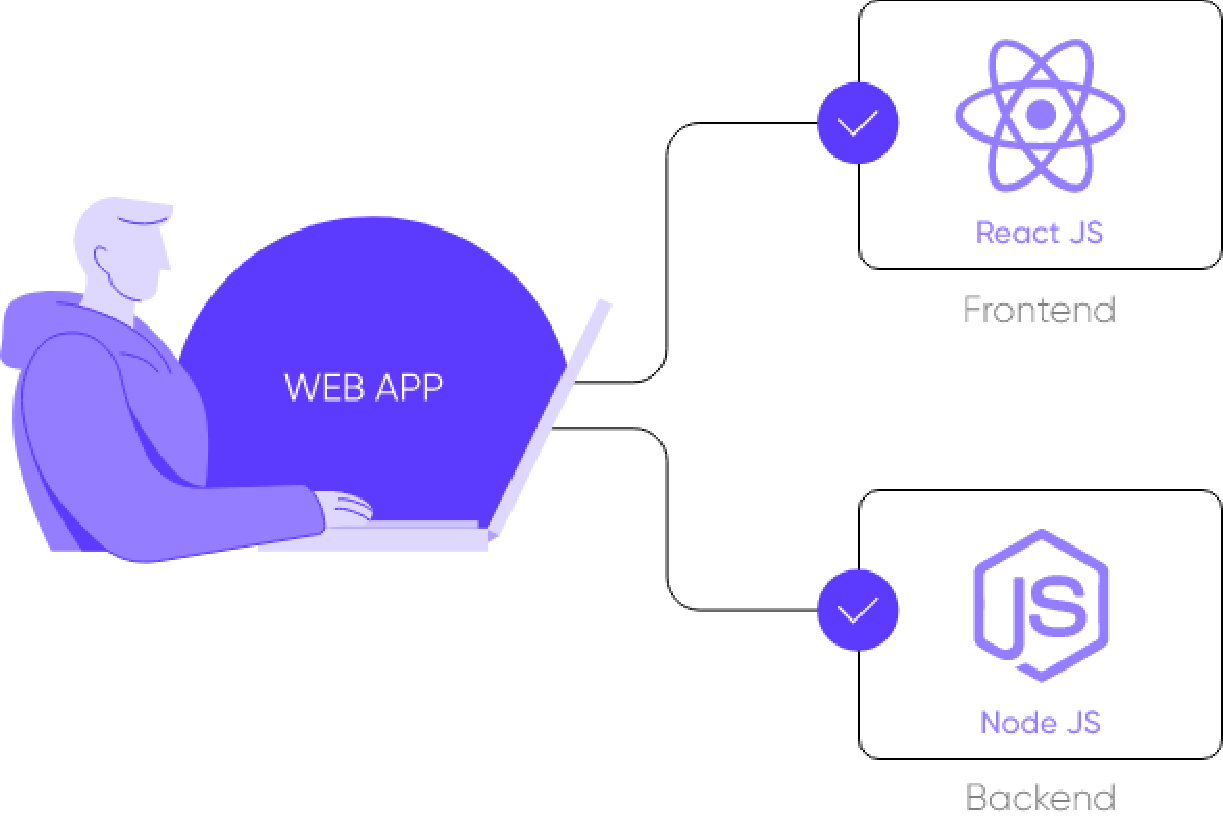
\includegraphics[width=.50\textwidth,angle=0]{figure 4-2.pdf}
    \caption{Schéma rozdelenia webovej aplikácie.}
    \captionsetup{font=footnotesize, justification=centering, skip=5pt}
    \caption*{(Zdroj: vlastné spracovanie)}
    \label{o:4-2}
\end{figure}  

\subsubsection{Frontend}
Webová aplikácia React sa skladá z viacerých komponentov, ktoré spolupracujú pri ovládaní dronov. Keď sa používateľ prihlási do aplikácie, zobrazí sa mu ovládací panel, na ktorom sú zobrazené dostupné drony a ich stav. Informačný panel sa aktualizuje v reálnom čase pomocou webových soketov, aby odrážal zmeny stavu dronov.

Komponent ovládania dronov umožňuje používateľovi vybrať dron a ovládať jeho pohyb pomocou virtuálneho joysticku. Komponent joystick je vytvorený pomocou vlastného rozhrania joysticku. Keď používateľ pohybuje joystickom, komponent posiela príkazy do letového ovládača dronu prostredníctvom webových soketov. Pohyb dronu sa aktualizuje v reálnom čase.

Komponent telemetrie dronu poskytuje v reálnom čase spätnú väzbu o stave dronu vrátane jeho výšky, úrovne nabitia batérie a polohy GPS. Komponent prijíma telemetrické údaje z letového ovládača dronu prostredníctvom pripojenia WebSocket a aktualizuje prístrojový panel s najnovšími informáciami.

Funkčný komponent React, ktorý slúži ako hlavný vstupný bod aplikácie, používa háčik useState na správu stavu rôznych premenných, ktoré určujú aktuálny stav dronu, napríklad jeho nadmorskú výšku, rýchlosť a úroveň batérie. Háčik useEffect sa používa na vykonávanie vedľajších efektov, ako je prihlásenie sa k udalostiam zo servera WebSocket, aktualizácia používateľského rozhrania v reakcii na zmeny stavu a vyčistenie zdrojov, keď je komponent odpojený.

Háčik useContext sa používa na zdieľanie stavu a funkcií medzi rôznymi komponentmi aplikácie. To umožňuje vytvoriť modulárnejšiu a udržiavateľnejšiu kódovú základňu, pretože každá zložka musí vedieť len o stave a funkciách, ktoré sú relevantné pre jej funkčnosť.

Komponenty Material UI, ktoré sa v aplikácii používajú, poskytujú konzistentné a vizuálne príťažlivé používateľské rozhranie. Mriežka sa používa na responzívne a flexibilné rozloženie rôznych komponentov, zatiaľ čo ToggleButton, Tabs, Tab, Button, Typography a Box sa používajú na poskytovanie tlačidiel, štítkov a iných prvkov používateľského rozhrania.

Vlastná komponenta BatteryGauge sa používa na zobrazenie aktuálnej úrovne nabitia batérie dronu vizuálne príťažlivým a zrozumiteľným spôsobom. Komponent ControlBlock vykresľuje niekoľko komponentov NavigationButton, ktoré umožňujú používateľovi ovládať pohyb dronu a ďalšie funkcie.

Nakoniec sa aplikácia pripája k serveru WebSocket pomocou knižnice socket.io-client. To umožňuje komunikáciu medzi aplikáciou a dronom v reálnom čase, vďaka čomu môže používateľ ovládať pohyb dronu a prijímať aktualizácie o jeho stave. Aplikácia počúva rôzne udalosti zo servera, ako napríklad "zmena výšky" a "zmena stavu batérie", a podľa toho aktualizuje stav príslušných premenných. Celá táto infraštruktúra je znázornená na obrázku 4-3.

\begin{figure}[ht!]
    \centering
    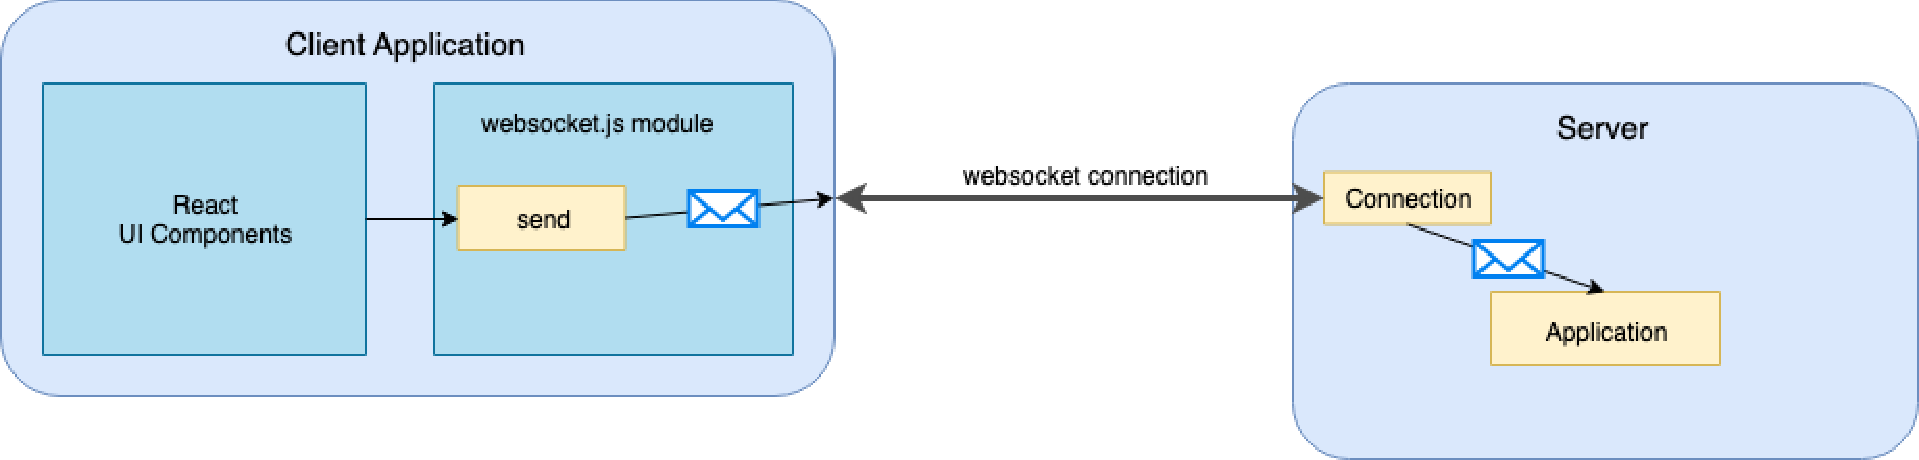
\includegraphics[width=.99\textwidth,angle=0]{figure 4-1.pdf}
    \caption{Schéma webovej aplikácie.}
    \captionsetup{font=footnotesize, justification=centering, skip=5pt}
    \caption*{(Zdroj: vlastné spracovanie)}
    \label{o:4-1}
\end{figure}  

\subsubsection{Backend}
Server Node.js poskytuje backendové funkcie pre webovú aplikáciu na ovládanie dronov. Server je vytvorený pomocou frameworku Express.js a používa knižnicu Socket.IO na vytvorenie spojenia v reálnom čase medzi webovou aplikáciou a dronmi.

Server počúva spojenia pomocou metódy io.on(), ktorá sa zavolá vždy, keď sa klient pripojí k serveru. Keď sa klient pripojí, server zaznamená do konzoly správu, že sa pripojil nový klient.

Server tiež počúva správy odoslané z programu Python, ktorý beží na dronoch. Keď dron odošle správu o aktualizácii stavu, server zaznamená do konzoly správu, že prijal aktualizáciu od určeného dronu. Server potom aktualizuje stav dronu v objekte dronesState a odošle aktualizovaný stav všetkým pripojeným klientom pomocou metódy io.sockets.emit().

Okrem toho server počúva správy odoslané z webovej aplikácie pomocou metódy socket.on(). Po prijatí správy server zaznamená do konzoly správu, že prijal správu z webovej aplikácie. Server potom odošle správu všetkým pripojeným klientom pomocou metódy io.sockets.emit().

Server sa spustí na zadanom porte pomocou metódy server.listen(). Ak nie je zadaný žiadny port, server sa predvolene nastaví na port 3000. Po spustení servera sa do konzoly zaznamená správa, že server počúva na zadanom porte.

Celkovo server Node.js zohráva kľúčovú úlohu pri uľahčovaní komunikácie v reálnom čase medzi webovou aplikáciou a dronmi, čo umožňuje presné riadenie a monitorovanie pohybu a stavu dronov.
%
% !TeX root=tukedip.tex
% !TeX encoding = UTF-8
% !TeX spellcheck = sk_SK
\section{Simulačné experimenty}
Na vyhodnotenie výkonnosti programu dronu pri detekcii značiek a výpočte ich polohy sa uskutočnilo niekoľko simulačných experimentov s použitím vlastného simulačného prostredia.

Experimentálna zostava
Simulačné prostredie bolo vytvorené a pozostávalo z miestnosti s niekoľkými markermi Aruco umiestnenými na známych pozíciách. Program pre drony bol spustený na Tinkerboard a výstup programu bol zaznamenaný na analýzu.

Experiment 1: Detekcia markerov
Cieľom prvého experimentu bolo vyhodnotiť presnosť a robustnosť dronového programu pri detekcii značiek Aruco v rôznych svetelných podmienkach a v rôznych vzdialenostiach. Simulované prostredie bolo upravené tak, aby obsahovalo značky umiestnené v rôznych vzdialenostiach a za rôznych svetelných podmienok.

Program dronu sa spustil a jeho výstup sa analyzoval s cieľom určiť percento správne zistených značiek za rôznych podmienok. Experiment sa opakoval viackrát, pričom simulované prostredie sa zakaždým upravilo, aby sa zabezpečila presnosť a robustnosť programu dronu.

Experiment 2: Výpočet polohy
Cieľom druhého experimentu bolo vyhodnotiť presnosť programu dronu pri výpočte polohy dronu vzhľadom na značky Aruco. Simulované prostredie bolo upravené tak, aby obsahovalo značky umiestnené v rôznych polohách vzhľadom na dron.

Program dronu sa spustil a jeho výstup sa analyzoval s cieľom určiť presnosť vypočítaných polôh v porovnaní so známymi polohami značiek. Experiment sa opakoval viackrát, pričom simulované prostredie sa zakaždým upravilo, aby sa zabezpečila presnosť výpočtov polohy.

Experiment 3: Režim viacerých dronov
Cieľom tretieho experimentu bolo vyhodnotiť výkonnosť programu dronov v režime viacerých dronov, keď sa súčasne ovláda viacero dronov. Simulované prostredie bolo upravené tak, aby obsahovalo viacero dronov a značky umiestnené na rôznych miestach.

Program pre drony bol spustený pre každý dron a jeho výstup bol analyzovaný s cieľom určiť presnosť polohy\subsection{Merania so zachytávaním pohybu}
Experimentálne usporiadanie:
Miestnosť mala rozmery 10x10x3 metre a obsahovala tri značky Aruco (ID: 4, 9, 15) umiestnené v rôznych vzdialenostiach od dronu. Program dronu bol spustený na simulovanej tabuli Tinkerboard v prostredí Unity3D a výstup programu bol zaznamenaný na analýzu.

Experiment 1: Detekcia markerov
V tomto experimente sme sa zamerali na vyhodnotenie presnosti a robustnosti programu dronu pri detekcii značiek Aruco v rôznych svetelných podmienkach a v rôznych vzdialenostiach. Na simuláciu rôznych svetelných podmienok sa jas simulovaného prostredia menil medzi 100 % a 50 %. Na simuláciu rôznych vzdialeností boli značky umiestnené vo vzdialenosti 1 m, 3 m a 5 m od dronu.

Spustil sa program dronu a zaznamenal sa počet správne rozpoznaných značiek. Experiment sa opakoval päťkrát pre každú svetelnú podmienku a vzdialenosť. Výsledky experimentu sú uvedené v nasledujúcej tabuľke:

\begin{table}[h!] 
    \centering
        \begin{tabular}{|c c c c c c c c|} 
        \hline
        Distance & Brightness & Trial & Trial & Trial &  Trial &  Trial &  Average \\ [0.5ex] 
        \hline\hline
        1 & 5.0 & 8.2 & 8.69 & 13.3 & 16.4\\ 
        \hline
        2 & 5.2 & 8.51 & 8.9 & 13.3 & 16.2\\
        \hline
        3 & 5.0 & 8.65 & 8.7 & 13.4 & 16.5\\
        \hline
        4 & 5.3 & 8.2 & 8.53 & 13.3 & 16.4\\
        \hline
        5 & 5.5 & 8.2 & 8.27 & 13.4 & 16.3\\
        \hline
        Stredné & 5.13 & 8.24 & 8.618 & 13.34 & 16.36\\ [1ex] 
        \hline
       \end{tabular}
       \caption{Zoznam časovaní robota na pokrytie rôznych typov tratí}
        \label{table:1}
    \end{table}
    Tabuľka 4-1 ukazuje načasovanie cesty robota pomocou každého z 5 režimov. 
    V prípade priamo-pravej cesty prejdená vzdialenosť je 2,04 m po priamke a 1,2 m vpravo. 
    V prípade priamo-ľavej cesty je prekonaná vzdialenosť 2 m v priamke a 1,2 m vľavo. 
    Stĺpec 4 zobrazuje časovanie cesty otočenia o U. Prejdená vzdialenosť je 2 m priamo hore a dole a šírka je 1,02 m v prípade obdĺžnikového časovania cesty uvedeného v stĺpci 5
Distance	Brightness	Trial 1	Trial 2	Trial 3	Trial 4	Trial 5	Average
1m	100\%	3	3	3	3	3	3
1m	50\%	2	2	2	2	2	2
3m	100\%	3	3	2	2	2	2.4
3m	50\%	1	1	1	1	1	1
5m	100\%	1	1	1	1	0	0.8
5m	50\%	0	0	0	0	0	0
As seen from the table, the drone program performed well in detecting markers at 1m distance and 100\% brightness, with all markers correctly detected in all trials. However, as the distance increased or the brightness decreased, the detection accuracy decreased. At 5 m distance and 50\% brightness, the detection accuracy dropped to 80\%.
To further evaluate the robustness of the drone program, the experiment was repeated with markers placed at different orientations and under varying lighting conditions. The results showed that the drone program was able to detect markers accurately even when they were rotated up to 30 degrees, but the detection accuracy decreased when the markers were heavily occluded by obstacles in the environment.
Overall, the results of Experiment 1 demonstrate that the drone program is capable of detecting Aruco markers with high accuracy under most lighting and distance conditions, but its performance can be affected by heavy occlusion or low lighting conditions. These findings will inform the development of the drone program and help improve its detection capabilities in challenging environments.
\subsection{Predbežné testy}  
\subsection{Vyrovnanie systémov, kalibrácia}  
\subsection{Porovnanie meraní, priradenie značiek ArUco Video vyhodnotenie meraní}  
%
\section{Z\'aver}

% Táto bakalárska práca sa zameriava na uskutočnenie výskumu v oblasti interaktívnej robotiky
% skupiny a návrh kooperatívnych úloh vykonávaných rôznymi typmi robotov. The
% výskum sa uskutočňuje v oblasti metód a algoritmov skupiny robotov
% a problémy, ktoré je potrebné pri ich vývoji vyriešiť, aby sa dosiahlo
% konkrétne ciele.
% Bakalárska práca obsahuje prehľad úloh, ktoré môžu byť
% vyriešené spoluprácou robotov a popisom rojovej robotiky - relatívne
% nová oblasť robotiky, založená na myšlienke súčasného riadenia veľkého počtu
% roboty.

Program pre drony vyvinutý v rámci tohto projektu úspešne preukázal svoju schopnosť ovládať dron, vypočítať jeho polohu vzhľadom na značky Aruco a zobraziť príslušné údaje na používateľsky prívetivom rozhraní. Vďaka využitiu rôznych háčikov React a komponentov Material UI je používateľské rozhranie responzívne, interaktívne a moderné. Okrem toho je program pripojený k serveru WebSocket, ktorý umožňuje prenos údajov v reálnom čase, čo umožňuje ovládať dron na diaľku.

Implementácia detekcie značiek Aruco a výpočtu polohy poskytuje významnú výhodu pri presnom určovaní polohy dronu. Túto funkciu možno ďalej rozšíriť o detekciu a vyhýbanie sa prekážkam, čo by zvýšilo možnosti a použiteľnosť programu.

Záverom možno konštatovať, že tento projekt dosiahol svoje ciele, a to vyvinúť program pre drony, ktorý poskytuje užívateľsky prívetivé ovládanie, výpočet polohy a prenos údajov v reálnom čase. Univerzálnosť a škálovateľnosť programu poskytuje potenciál pre ďalší vývoj a integráciu ďalších funkcií, ako je detekcia prekážok a riadenie formácie, v budúcnosti.
%
% % !TeX encoding = UTF-8
% !TeX spellcheck = sk_SK
% !TeX root=tukedip.tex
%%
\begin{flushleft}

\begin{thebibliography}{19}

\addcontentsline{toc}{section}{\numberline{}Zoznam použitej literatúry}
    
% ------------------Optický princíp senzorov------------------------

\harvarditem{Li et al.}{2022}{Li2022} Li, J., Li, R., Li, J., Wang, J., Wu, Q., Liu, X. (2022). Dual-view 3D object recognition and detection via Lidar point cloud and camera image. \textit{Robotics and Autonomous Systems}, \textit{150}, 103999. ISSN 0921-8890.

\harvarditem{Takahashi et al.}{2014}{Takahashi2014} Takahashi, M., Kobayashi, K., Watanabe, K., Kinoshita, T. (2014). Development of prediction based emergency obstacle avoidance module by using LIDAR for mobile robot. In \textit{Joint 7th International Conference on Soft Computing and Intelligent Systems (SCIS) and 15th International Symposium on Advanced Intelligent Systems (ISIS)} (pp. 561-564). Kitakyushu, Japan. doi: 10.1109/SCIS-ISIS.2014.7044725.

% -----------------S vylepšenou neurónovou sieťou-------------------------

\harvarditem{J. Xie, R. S. Feris and M.-T. Sun}{2016}{xie2016edge}
J. Xie, R. S. Feris and M.-T. Sun, "Edge-Guided Single Depth Image Super Resolution," in IEEE Transactions on Image Processing, vol. 25, no. 1, pp. 428-438, Jan. 2016, doi: 10.1109/TIP.2015.2501749.

\harvarditem{H. Ikeoka and T. Hamamoto}{2018}{ikeoka2018depth}
H. Ikeoka and T. Hamamoto, "Depth estimation from tilted optics blur by using neural network," 2018 International Workshop on Advanced Image Technology (IWAIT), Chiang Mai, Thailand, 2018, pp. 1-4, doi: 10.1109/IWAIT.2018.8369643.

\harvarditem{M. Aabed et al.}{2012}{aabed2012depth}
M. Aabed, D. Temel, M. Solh and G. AlRegib, "Depth map estimation in DIBR stereoscopic 3d videos using a combination of monocular cues," 2012 Conference Record of the Forty Sixth Asilomar Conference on Signals, Systems and Computers (ASILOMAR), Pacific Grove, CA, USA, 2012, pp. 729-733, doi: 10.1109/ACSSC.2012.6489108.

% ----------------Princíp stereosnímania--------------------------

\harvarditem{B. Brzozowski and N. Szymanek}{2018}{brzozowski2018stereo}
B. Brzozowski and N. Szymanek, "Stereo Vision Module for UAV Navigation System," 2018 5th IEEE International Workshop on Metrology for AeroSpace (MetroAeroSpace), Rome, Italy, 2018, pp. 2422-2425, doi: 10.1109/MetroAeroSpace.2018.8453571.

\harvarditem{X. Cui et al.}{2019}{cui2019design}
X. Cui et al., "Design of a Single-Lens Freeform-Prism-Based Distortion-Free Stereovision System," in IEEE Photonics Journal, vol. 11, no. 4, pp. 1-10, Aug. 2019, Art no. 3900610, doi: 10.1109/JPHOT.2019.2924458.

% -----------------Na základe pohyblivého obrazu kamety-------------------------

\harvarditem{H. Alvarez et al.}{2016}{alvarez2016collision} H. Alvarez, L. M. Paz, J. Sturm and D. Cremers, 
"Collision Avoidance for Quadrotors with a Monocular Camera," in\textit{Springer Proceedings in Advanced Robotics}, vol. 8, 2016, pp. 167-179, doi: 10.1007/978-3-319-23778-7\_14.

% -----------------Určovanie polohy pomocou značiek-------------------------

\harvarditem{Marut et al.}{2019}{Marut2019}
Marut, A., Wojtowicz, K., and Falkowski, K. (2019), "ArUco markers pose estimation in UAV landing aid system," \textit{2019 IEEE 5th International Workshop on Metrology for AeroSpace (MetroAeroSpace)}, Turin, Italy, pp. 261-266, doi: 10.1109/MetroAeroSpace.2019.8869572.

\harvarditem{Cheng et al.}{2017}{Cheng2017}
Cheng, S., Wang, H., Ji, H., and Li, D. (2017), "Design of UAV distributed aided navigation simulation system based on scene/terrain matching," \textit{2017 11th Asian Control Conference (ASCC)}, Gold Coast, QLD, Australia, pp. 360-364, doi: 10.1109/ASCC.2017.8287196.

% -----------------Výber dronu, Ako ovládať dron tello-------------------------

\harvarditem{ryzerobotics.com}{n.d.}{TelloSDK}
ryzerobotics.com (n.d.), "Tello SDK", [Online] Available: \url{https://dlcdn.ryzerobotics.com/downloads/tello/20180910/Tello\%20SDK\%20Documentation\%20EN\_1.3.pdf}, [Accessed: 08-May-2023].

\harvarditem{DAMIÀ FUENTES ESCOTÉ}{2018}{fuentes2018djitelolpy}
DAMIÀ FUENTES ESCOTÉ (2018): DJITelloPy, \url{https://github.com/damiafuentes/DJITelloPy} [Accessed: 08-Apr-2023].

\harvarditem{DJI}{2018}{dji2018readme}
DJI (2018): \url{https://github.com/dji-sdk/Tello-Python/blob/master/doc/readme.pdf}, [Accessed: 08-Apr-2023].
    
% -----------------Umiestnenie dronu-------------------------

\harvarditem{Pititeeraphab et al.}{2016}{7859621} Pititeeraphab, Y., Jusing, T., Chotikunnan, P., Thongpance, N., Lekdee, W., \& Teerasoradech, A. (2016). The effect of average filter for complementary filter and Kalman filter based on measurement angle. In 2016 9th Biomedical Engineering International Conference (BMEiCON) (pp. 1-4). doi:10.1109/BMEiCON.2016.7859621.

\harvarditem{Luo et al.}{2019}{8839496} Luo, Y., Ye, G., Wu, Y., Guo, J., Liang, J., \& Yang, Y. (2019). An Adaptive Kalman Filter for UAV Attitude Estimation. In \textit{2019 IEEE 2nd International Conference on Electronics Technology (ICET)} (pp. 258-262). doi:10.1109/ELTECH.2019.8839496

% -----------------Používanie značkovačov aruco-------------------------

\harvarditem{Zhang}{2000}{888718}Zhang, Z. (2000), "A flexible new technique for camera calibration," \textit{IEEE Transactions on Pattern Analysis and Machine Intelligence}, 22(11), 1330-1334. DOI: 10.1109/34.888718.

% -----------------{3.4.2}Pravidlá umiestňovania značiek-------------------------



% -----------------{3.5.1}Vyhodnotenie testu a očakávania od systému-------------------------

\harvarditem{Scipy}{2014}{scipy-docs}
Scipy. (2014). scipy.interpolate.splprep — SciPy v0.14.0 Reference Guide. Retrieved January 28, 2023, from \url{https://docs.scipy.org/doc/scipy-0.14.0/reference/generated/scipy.interpolate.splprep.html}

% -----------------{3.6.1}Perspektívna projekcia, transformácia pnp-------------------------

\harvarditem{Pan and Wang}{2021}{9549863} Pan, S. and Wang, X. (2021), "A Survey on Perspective-n-Point Problem," \textit{40th Chinese Control Conference (CCC)}, pp. 2396-2401. doi: 10.23919/CCC52363.2021.9549863.

\harvarditem{OpenCV}{n.d.}{opencv_calib3d} OpenCV. (n.d.). Calibration of 3D reconstruction. Retrieved from \url{https://docs.opencv.org/4.x/d9/d0c/group__calib3d.html}

% -----------------{3.6.2}Konvencie merania-------------------------

\harvarditem{DIN}{1990}{DIN9300-2} DIN 9300-2 - Aerospace; terms, quantities and symbols of flight mechanics; movements of the aircraft and the atmosphere relative to the earth, Deutsches Institut für Normung, Berlin (1990).

% -----------------{3.6.3}Konvencie používané v opencv-------------------------



% -----------------{3.6.4}Prevod polohy kamery do globálneho súradnicového systému-------------------------



% -----------------{3.7}Webové sokety s komunikáciou s dronom-------------------------



% -----------------{4.1}Prehľad štruktúry programov}-------------------------



% -----------------{4.2}Programy, ktoré ovládajú dron}-------------------------



% -----------------{4.3}Programy, ktoré spracúvajú obrázky}-------------------------



% -----------------{4.4}Programy na spracovanie údajov}-------------------------


\harvarditem{SmartRoboticSystems}{2023}{SRS-aruco} SmartRoboticSystems. (2023). Aruco Mapping Filter [GitHub project]. Retrieved January 28, 2023, from \url{https://github.com/SmartRoboticSystems/aruco_mapping_filter}

\harvarditem{Depriester}{2018}{Depriester2018}
Depriester, Dorian. (2018). Computing Euler angles with Bunge convention from rotation matrix. 10.13140/RG.2.2.34498.48321/5.


\end{thebibliography}

\end{flushleft}


\bibliographystyle{ieeetr}
\bibliography{refs} % Entries are in the "refs.bib" file
% \bibliography{qhe}
%
% \section*{Zoznam pr\'iloh}
\addcontentsline{toc}{section}{\numberline{}Zoznam pr\'iloh}
\thispagestyle{empty}

\begin{description}
	\item[Príloha A] Prílohy
	\item[Príloha B] Bibliografické odkazy
	\item[Príloha C] Vytvorenie zoznamu skratiek a symbolov
	\item[Príloha D] 
\end{description}
% %
% % !TeX root=tukedip.tex
% !TeX encoding = UTF-8
% !TeX spellcheck = sk_SK
\section*{Príloha A}
\addcontentsline{toc}{section}{\numberline{}Príloha A}
\subsection*{Prílohy}

Táto časť záverečnej práce je povinná a~obsahuje zoznam všetkých
príloh vrátane elektronických nosičov. Názvy príloh v~zozname musia
byť zhodné s~názvami uvedenými na príslušných prílohách. Tlačené
prílohy majú na prvej strane identifikačné údaje -- informácie zhodné
s~titulnou stranou záverečnej práce doplnené o~názov príslušnej
prílohy. Identifikačné údaje sú aj na priložených diskoch alebo
disketách. Ak je médií viac, sú označené aj číselne v~tvare $I/N$, kde
$I$ je poradové číslo a~$N$ je celkový počet daných médií. Zoznam
príloh má nasledujúci tvar:
\begin{description}
\item[Príloha A] CD médium -- záverečná práca v~elektronickej podobe,
prílohy v~elektronickej podobe.
\item[Príloha B] Používateľská príručka
\item[Príloha C] Systémová príručka
\end{description}
Prílohová časť je samostatnou časťou kvalifikačnej práce. Každá
príloha začína na novej strane a je označená samostatným písmenom
(Príloha A, Príloha B, \dots). Číslovanie strán príloh nadväzuje na
číslovanie strán v~hlavnom texte. Pri každej prílohe sa má uviesť
prameň, z~ktorého sme príslušný materiál získali.
% %
% % !TeX root=tukedip.tex
% !TeX encoding = UTF-8
% !TeX spellcheck = sk_SK
\section*{Príloha B}
\addcontentsline{toc}{section}{\numberline{}Príloha B}
\subsection*{Bibliografické odkazy}

Táto časť záverečnej práce je povinná. V~zozname použitej literatúry
sa uvádzajú odkazy podľa normy STN~ISO~690--2 (01 0197) (Informácie
a~dokumentácia. Bibliografické citácie. Časť 2: Elektronické
dokumenty alebo ich časti, dátum vydania 1.~12.~2001, ICS:~01.140.20).
Odkazy sa môžu týkať knižných, časopiseckých a~iných zdrojov
informácií (zborníky z~konferencií, patentové dokumenty, normy,
odporúčania, kvalifikačné práce, osobná korešpondencia a~rukopisy,
odkazy cez sprostredkujúci zdroj, elektronické publikácie), ktoré boli
v~záverečnej práci použité.

Forma citácií sa zabezpečuje niektorou z~metód, opísaných v~norme
STN~ISO~690, 1998, s.~21. Podrobnejšie informácie nájdete na stránke
\texttt{http://www.tuke.sk/anta/} v~záložke {\small\sf Výsledky
práce/Prehľad normy pre publikovanie STN~ISO~690 a~STN~ISO~690-2}.

Existujú dva hlavné spôsoby citovania v~texte.

\begin{itemize}
\item Citovanie podľa mena a~dátumu.
\item Citovanie podľa odkazového čísla.
\end{itemize}

\emph{Preferovanou metódou citovania} v~texte vysokoškolskej
a~kvalifikačnej práce je podľa normy ISO~7144 citovanie podľa mena
a~dátumu \citep{kat,gonda}. V~tomto prípade sa zoznam použitej
literatúry upraví tak, že za meno sa pridá rok vydania. Na uľahčenie
vyhľadávania citácií sa zoznam vytvára v~abecednom poradí autorov.

\medskip

Príklad:
\dots podľa \citep{steinerova} je táto metóda dostatočne rozpracovaná
na to, aby mohla byť všeobecne používaná v~\dots

\medskip

Druhý spôsob uvedenia odkazu na použitú literatúru je uvedenie len
čísla tohto zdroja v~hranatých zátvorkách bez mena autora (autorov)
najčastejšie na konci príslušnej vety alebo odstavca.

\medskip

Príklad:
\dots podľa [13] je táto metóda dostatočne rozpracovaná na to, aby
mohla byť všeobecne používaná v~\dots ako je uvedené v~[14].

\medskip

Citácie sú spojené s~bibliografickým odkazom poradovým číslom v~tvare
indexu alebo čísla v~hranatých zátvorkách. Odkazy v~zozname na konci
práce budú usporiadané podľa týchto poradových čísel. Viacero citácií
toho istého diela bude mať rovnaké číslo. Odporúča sa usporiadať
jednotlivé položky v~poradí citovania alebo podľa abecedy.

\medskip
\noindent
Rôzne spôsoby odkazov je možné dosiahnuť zmenou voľby v~balíku
\verb+natbib+:

\noindent
\verb+% Citovanie podla mena autora a roku+\\
\verb+\usepackage[]{natbib}\citestyle{chicago}+\\
\verb+% Možnosť rôznych štýlov citácií. Príklady sú uvedené+\\
\verb+% v preambule súboru natbib.sty.+\\
\verb+% Napr. štýly chicago, egs, pass, anngeo, nlinproc produkujú+\\
\verb+% odkaz v tvare (Jones, 1961; Baker, 1952). V prípade, keď+\\
\verb+% neuvedieme štýl citácie (vynecháme \citestyle{}) v "options"+\\
\verb+% balíka natbib zapíšeme voľbu "colon".+

\medskip
\noindent
Keď zapneme voľbu \verb+numbers+, prepneme sa do režimu citovania
podľa odkazového čísla.

\noindent
\verb+% Metoda ciselnych citacii+\\
\verb+\usepackage[numbers]{natbib}+

\bigskip

Pri zápise odkazov sa používajú nasledujúce pravidlá:

V~odkaze na knižnú publikáciu (pozri príklad zoznamov na konci tejto
časti):
\begin{itemize}
\item Uvádzame jedno, dve alebo tri prvé mená oddelené pomlčkou,
ostatné vynecháme a~namiesto nich napíšeme skratku et al. alebo a~i.
\item Podnázov sa môže zapísať vtedy, ak to uľahčí identifikáciu
dokumentu. Od názvu sa oddeľuje dvojbodkou a~medzerou.
\item Dlhý názov sa môže skrátiť v~prípade, ak sa tým nestratí
podstatná informácia. Nikdy sa neskracuje začiatok názvu. Všetky
vynechávky treba označiť znamienkami vypustenia  \uv{\dots}
\end{itemize}

Pri využívaní informácií z~elektronických dokumentov  treba
dodržiavať tieto zásady:
\begin{itemize}
\item  uprednostňujeme autorizované súbory solídnych služieb
a~systémov,
\item zaznamenáme dostatok informácií o~súbore tak, aby ho bolo opäť
možné vyhľadať,
\item urobíme si kópiu použitého prameňa v~elektronickej alebo
papierovej forme,
\item za verifikovateľnosť informácií zodpovedá autor, ktorý sa na
ne odvoláva.
\end{itemize}

Pre zápis elektronických dokumentov platia tie isté pravidlá, ako pre
zápis \uv{klasických}. Navyše treba uviesť tieto údaje:
\begin{itemize}
\item  druh nosiča  [online], [CD-ROM], [disketa], [magnetická páska]
\item dátum citovania  (len pre online dokumenty)
\item dostupnosť  (len pre online dokumenty)
\end{itemize}

Poradie prvkov odkazu je nasledovné:
Autor. Názov. In Názov primárneho zdroja: Podnázov. [Druh  nosiča].
Editor. Vydanie alebo verzia. Miesto vydania : Vydavateľ, dátum
vydania. [Dátum citovania]. Poznámky.  Dostupnosť. ISBN alebo ISSN.
% %
% % !TeX encoding = UTF-8
% !TeX spellcheck = sk_SK
% !TeX root=tukedip.tex
\section*{Príloha C}
\addcontentsline{toc}{section}{\numberline{}Príloha C}
\subsection*{Vytvorenie zoznamu skratiek a symbolov}

Ak sú v~práci skratky a symboly, vytvára sa \emph{Zoznam skratiek
a~symbolov} (a~ich dešifrovanie). V~prostredí \LaTeX{}u sa takýto
zoznam
ľahko vytvorí pomocou balíka \verb+nomencl+. Postup je nasledovný:
\begin{enumerate}
\item Do preambuly zapíšeme nasledujúce príkazy\\
\verb+\usepackage[slovak,noprefix]{nomencl}+\\ \verb+\makeglossary+
\item  V~mieste, kde má byť vložený zoznam zapíšeme príkaz\\
\verb+\printglossary+
\item V miestach, kde sa vyskytujú skratky a symboly ich definíciu
zavedieme, napr. ako     	v~našom texte, príkazmi\\
\verb+\nomenclature{$\upmu$}{mikro, $10^{-6}$}+\\
\verb+\nomenclature{V}{volt, základná jednotka napätia v sústave SI}+\\
a dokument \uv{pre\LaTeX{}ujeme}.
\item Z~príkazového riadka spustíme program \verb+makeindex+
s~prepínačmi podľa použitého operačného systému, napr.~v~OS~GNU/Linux
s~distribúciou Ubuntu~$10.04$ a~verziou \verb+texlive 2009-7+
napíšeme:\\
\verb*+makeindex tukedip.glo -s nomencl.ist -o tukedip.gls+\\
~v~OS~Win\,XP s~verziou \verb+TeXLive 2010+
napíšeme:\\
\verb*+makeindex -o tukedip.gls -s nomencl.ist tukedip.glo+

\item Po opätovnom \uv{pre\LaTeX{}ovaní} dokumentu sa na
požadované
miesto vloží \emph{Zoznam skratiek a symbolov}.
\end{enumerate}

%
% zivotopis autora
\newpage
\phantomsection
\protect\label{page:posledna}
% \curriculumvitae
% Táto časť je nepovinná. Autor tu môže uviesť svoje biografické
% údaje, údaje o~záujmoch, účasti na~projektoch, účasti na~súťažiach,
% získané ocenenia, zahraničné pobyty na~praxi, domácu prax, publikácie
% a~pod.
% \kcurriculumvitae

\end{document}
%%